%%%%%%%%%%%%%%%%%%%%%%%%%%%%%%%%%%%%%%START PREAMBLE 
\documentclass{article}
%\usepackage{Sweave}
\usepackage{graphicx}
\usepackage{tabularx}
\usepackage{hyperref}
\usepackage{natbib}
\usepackage{pdflscape}
\usepackage{array}
\usepackage{authblk}
\usepackage{gensymb}

\usepackage[small]{caption}

\setkeys{Gin}{width=0.8\textwidth} %make the figs 50 perc textwidth
\setlength{\captionmargin}{30pt}
\setlength{\abovecaptionskip}{10pt}
\setlength{\belowcaptionskip}{10pt}
\topmargin -1.5cm    
\oddsidemargin -0.04cm  
\evensidemargin -0.04cm % same as oddsidemargin but for left-hand pages
\textwidth 16.59cm
\textheight 21.94cm 
%\pagestyle{empty}    % Uncomment if don't want page numbers
\parskip 7.2pt      % sets spacing between paragraphs
\parindent 0pt% sets leading space for paragraphs
\usepackage{setspace}
\renewcommand{\baselinestretch}{1.8}
\usepackage{lineno}
%%%%%%%%%%%%%%%%%%%%%%%%%%%%%%%%%%%%%%END PREAMBLE THAT IS THE SAME FOR ALL EXAMPLES

%Start of the document
\begin{document}

%\Sconcordance{concordance:photoperiod.tex:photoperiod.Rnw:%
1 249 1}


\bibliographystyle{ecology.bst}
\title{Spatial and temporal shifts in photoperiod with climate change} % perspective paper for OSPREE analyses


\author[1,2,a]{A. K. Ettinger (ailene.ettinger@tnc.org, ORCID ID:  0000-0002-6228-6732, twitter: @AileneKane)}
\author[2,3]{D. M. Buonaiuto (dbuonaiuto@g.harvard.edu, ORCID ID: 0000-0003-4022-2591)}

\author[2,3]{C. J. Chamberlain (cchamberlain@g.harvard.edu, ORCID ID: 0000-0001-5495-3219)}

\author[2,3,4,5]{I. Morales-Castilla (ignacio.moralesc@uah.es, ORCID ID: 0000-0002-8570-9312, twitter: @GloCEE\_EcoEvo)}

\author[2,3,6]{E. M. Wolkovich (e.wolkovich@ubc.ca, ORCID ID: 0000-0001-7653-893X)}

\affil[1]{The Nature Conservancy, Seattle, Washington, USA 98121}

\affil[2]{Arnold Arboretum of Harvard University, Boston, Massachusetts, USA 02130}


\affil[3]{Department of Organismic and Evolutionary Biology, Harvard University, Cambridge, Massachusetts, USA 02138}

\affil[4]{Department of Life Sciences, University of Alcal\`a CTRA N-II, KM., 33,600, 28802, Alcal\`a de Henares, Spain}

\affil[5]{Department of Environmental Science and Policy, George Mason University, Fairfax, Virginia, USA 22030}
 
\affil[6]{Forest \& Conservation Sciences, Faculty of Forestry, University of British Columbia, Vancouver, British Columbia, Canada V6T 1Z4}

\affil[a]{Corresponding author; phone: 781-296-4821; mailing address: 74 Wall Street, Seattle, WA 98121 USA}

\date{Article acceptance date: December 8, 2020} 

\maketitle %put the fancy title on
\textbf{Statement of authorship} 
All authors conceived of this manuscript and each contributed data analysis and figures. AKE wrote the manuscript, and all authors contributed revisions to the manuscript. 

\textbf{Data Accessibility} The OSPREE database is publicly archived at KNB, doi:10.5063/F1CZ35KB. \citep{wolkovich2019}.

\textbf{Running head} Shifts in photoperiod with climate change

\textbf{Key words} phenology, global warming, range shifts, timing, spring, budburst,daylength 

\textbf{Paper type} `Research review' or `Viewpoint'


%%%%%%%%%%%%%%%%%%%%%%%%%%%%%%%%%%%%%%%%%%%%%%%%%%%

%%%%%%%%%%%%%%%%%%%%%%%%%%%%%%%%%%%%%%%%%%%%%%%%%%%
\newpage
\linenumbers
\section*{Abstract}
Climate change causes both temporal (e.g., advancing spring phenology) and geographic (e.g., range expansion poleward) species shifts, which affect the photoperiod experienced at critical developmental stages (`experienced photoperiod'). As photoperiod is a common trigger of seasonal biological responses---affecting woody plant spring phenology in 87\% of reviewed studies that manipulated photoperiod---shifts in experienced photoperiod may have important implications for future plant distributions and fitness. However, photoperiod has not been a focus of climate change forecasting to date, especially for early-season (`spring') events, often assumed to be driven by temperature. Synthesizing published studies, we find that impacts on experienced photoperiod from temporal shifts could be orders of magnitude larger than from spatial shifts (1.6 hours of change for expected temporal versus one minute for latitudinal shifts). Incorporating these effects into forecasts is possible by leveraging existing experimental data; we show that results from growth chamber experiments on woody plants often have data relevant for climate change impacts, and suggest that shifts in experienced photoperiod may increasingly constrain responses to additional warming. Further, combining modeling approaches and empirical work on when, where, and how much photoperiod affects phenology could rapidly advance our understanding and predictions of future spatio-temporal shifts from climate change. 

\newpage
\section*{Introduction}

\par Shifts in phenology---i.e., the timing of biological events, including budburst, leafout, and flowering in plants, as well as bird arrival, egg hatching and myriad other biological activities---are some of the most widely documented signals of climate change. Spring phenology in particular has shifted, occurring earlier as temperatures warm, with average shifts of 1.2 to 5.1 days earlier per decade \citep{bradley1999,parmesan2003, poloczanska2013,root2003} or 1.3 to 5.6 days earlier per \degree C of warming \citep{polgar2013,Wolkovich:2012n}. These changes are some of the largest climate change-induced shifts observed, with early spring phenology shifting more rapidly than later season phenology in most cases \citep{bradley1999,menzel2006}. 

\par Phenology is not controlled solely by temperature, however. Photoperiod is also a critical cue, signaling changes in growth and reproduction across diverse species \citep[e.g.,][]{flynn2018,lagercrantz2009,bradshaw2007,Howe:1996,solbakken1994}. Even spring phenology, which is highly temperature-sensitive, is thought to be determined interactively by photoperiod and temperature \citep[][see also Box 1]{fu2019}. Photoperiod is a useful cue to synchronize activities with seasonal climatic changes \citep[e.g.,][]{Singh:2017, Basler:2012, Hsu:2011} because it is consistent across years, especially compared to other cues such as temperature and precipitation \citep{saikkonen2012}.  For example, relying on a threshold photoperiod (see Table 1), rather than temperature alone, may prevent woody plants from leafing out during `false spring' events \citep[unusually warm periods during winter and early spring that are followed by a return to cold temperatures,][]{gu2008}. 

\par Recent studies suggest that photoperiod cues may eventually restrict phenology in a warmer world. With additional climate change, photoperiod may limit phenological shifts of certain species such that they will not track rising temperatures \citep{fu2015,way2015,Basler:2012,koerner2010a}. The idea of photoperiod constraints is controversial, however, as other studies suggest that photoperiod will not slow responses to warming for most species \citep{chuine2010,zohner2016}. Resolving this debate requires a greater understanding of the extent to which daylength constrains phenology and how rapidly photoperiod responses can acclimate or adapt to new environmental conditions \citep{grevstad2015}.

\par Perhaps because of these variable and uncertain responses, photoperiod is often not included in forecasts of biological responses to climate change, especially in the spring, even though it is known to be an important cue for biological activity \citep[but see ][]{duputie2015,grevstad2015,Caffarra:2011qf}. The exclusion of photoperiod may be problematic: although photoperiod itself is stable over time, the photoperiod that species \emph{experience} at critical developmental stages (henceforth, `experienced photoperiod'), as they undergo climate change-induced shifts in space and time, is likely to be much less stable (Fig. \ref{fig:spacetime}). This shift in experienced photoperiod extends to distributional shifts due to climate change, as many species' distributions have moved poleward and upward in elevation \citep[i.e., range shifts,][]{chen2011,harsch2009,parmesan2006,penuelas2003}. 
\par The implications of potential climate change-induced shifts in experienced photoperiod are unclear, as the magnitudes of potential shifts have not been described. Effects of photoperiod shifts may be relatively minor, especially compared to the substantial year-to-year variation in experienced photoperiod (Fig. \ref{fig:greenup}). Alternatively, photoperiod may begin to constrain species' responses to climate change \citep{huffeldt2020,fu2015,way2015,Basler:2012,koerner2010a}.

\par Here, we ask: 
\begin{enumerate}
\item How will climate change alter experienced photoperiod for plants? 
\item What are the implications of altered experienced photoperiods for plant responses to climate change?
\item Can researchers apply data from experiments that alter photoperiod to improve forecasts of biological implications of climate change?

\end{enumerate}
\par Our questions are broadly relevant for diverse species and seasonal events. We use a case study of spring woody plant phenology to illustrate several of our points (Boxes 1 \& 2). We focus on spring events, as phenology during this time is one of the most widely observed and rapidly changing biological responses to climate change \citep{parmesan2006}. In addition, the role of photoperiod is less understood in spring phenology compared with autumn phenophases \citep[reviewed in, e.g.,][]{azeez2015,gallinat2015,gill2015,lagercrantz2009, allona2008}, but recent studies showing declines in responses of spring budburst to warming \citep[e.g.,][]{fu2019,gusewell2017,yu2010} suggest that photoperiod constraints may be imminent. 

\section*{How will climate change alter experienced photoperiod for plants?}
\par Species experience different photoperiod regimes depending on their location on Earth, the seasonal timing of their activity, and inter-annual variation in climate (Fig. \ref{fig:spacetime}). Consider, as an example, the daylength experienced by plants on the date that spring `green-up' occurs. We use green-up date as an example because it represents an important spring event, signaling the start of the growing season, and global estimates are available. Photoperiod on green-up date varies with latitude (Fig. \ref{fig:greenup}A), in part because latitudinal variation in green-up date, which occurs earlier toward the equator and later toward the poles, is strongly driven by climatic differences that affect phenology, and in part because of latitudinal variation in photoperiod (e.g., at the poles, the daylength at the summer solstice is 24 hours; see also Fig. \ref{fig:spacetime}). (See ``Quantifying and mapping differences in green-up across the United States and Europe'' in the \emph{Methods S1} for additional details of this analysis.) 
\par Some consistent patterns in experienced photoperiod are apparent at a broad scale. Across years, photoperiod at green-up is longer toward the poles (i.e., on the day of year when green-up occurs close to the north pole, daylength approaches 24 hours in both an average year, Fig. \ref{fig:greenup}A, and in an early year, Fig. \ref{fig:greenup}B). In addition, green-up does not appear to occur at daylengths less than 10 hours across North America and Europe. 
\par Despite these consistent broad-scale patterns, there is also strong spatiotemporal variation in experienced photoperiod across years. Comparing the photoperiod at green-up in an `early' versus an `average' year (Fig. \ref{fig:greenup}A,B) shows that experienced photoperiod at green-up can vary by two to three hours from one year to the next in the same location (Fig. \ref{fig:greenup}C).

\par Against this existing background variation, climate change will cause shifts in experienced photoperiod as species respond to warming temperatures. Spatial shifts in species' ranges and temporal shifts in phenology will alter the photoperiods experienced by organisms with future climate change. The magnitude of these alterations will vary depending on the organism's location and the type of shift(s) it undergoes. For example, poleward shifts in species' ranges cause plants to experience a wider range of daylength throughout the year (Fig. \ref{fig:spacetime}), which may pose challenges to organisms undergoing temperature-induced poleward range shifts \citep{huffeldt2020}. Elevational shifts, in contrast, cause minimal change to the range of daylength throughout the year.

\par To date, most focus on shifts in photoperiod with climate change has centered on how spatial range shifts will affect photoperiod \citep[e.g.,][]{huffeldt2020,way2015,saikkonen2012}. However, shifting phenology---especially the large changes seen in spring phenology---will also alter experienced photoperiod, because of the seasonal patterns of daylength (Fig. \ref{fig:spacetime}). 

\par Current data suggest that temporal shifts will yield much larger changes in experienced photoperiod than latitudinal shifts (Fig. \ref{fig:spacetime}).
Consider a tree species that bursts its buds at latitude 45$^{\circ}$, on average around day of year 91 (April 2), when daylength is 12.8 hours. If the species' phenology shifts 30 days earlier over the next century \citep[i.e., a rate of ~3 days per decade, as has been observed,][]{parmesan2003}, it will experience a daylength that is 1.6 hours shorter. This 1.6 hour decrease in daylength is equivalent to moving up 28.5$^{\circ}$ in latitude on this day of year. However, if the same species shifts its range up in latitude 0.5$^{\circ}$ \citep[i.e., 60 km over the next century, comparable to observed rates,][]{chen2011,parmesan2003}, it will experience a daylength that differs by less than a minute on the same day of year. 
\par Temporal shifts in temperate areas are likely to yield larger changes in experienced photoperiod for autumn phenology, as well. Consider again the tree at latitude 45$^{\circ}$, which may senescence on day of year 300 (October 27), on average \citep{gill2015}, when daylength is 10.5 hours. If senescence shifts 33 days later over the next century \citep[i.e., a rate of 3.3 days per decade, as has been observed,][]{gill2015}, it will experience, at the end of the growing season, a daylength that is 1.3 hours shorter. This is equivalent to moving up 16$^{\circ}$ in latitude on this day of year.
\section*{What are the implications of altered photoperiods for plant responses to climate change?}
Climate change alters the experienced photoperiod, but the implications of this change for plants are currently unclear, in part, because phenology both affects and is affected by experienced photoperiod: climate change-induced shifts in phenology alter experienced photoperiod, which in turn affects phenology. Daylength, often in combination with temperature, can play a role in controlling critical biological functions, including vegetative growth, cell elongation, budburst, and flowering in plants \citep{fu2019,Heide:2012aa,Heide:2011aa,Hsu:2011,sidaway2010,mimura2007,Linkosalo:2006aa,erwin1998,Ashby:1962aa}.
Climate change-induced shifts in photoperiod are therefore likely to alter these functions. 

\par Growth chamber studies show that the magnitude of daylength shifts expected with climate change (i.e., 1-2 hours of difference in daylength with temporal shifts over the next century) are substantial enough to affect spring phenology in trees (Table S1). The direction and magnitude of responses will vary, however, because of variation in photoperiod sensitivity, and because photoperiod often interacts with other environmental drivers, such as temperature, to affect phenology (Box 1). 

\par The climate change-induced trend toward ever-earlier springs means that experienced photoperiod may increasingly approach threshold photoperiods (see Table 1) for many species, potentially constraining their ability to respond to additional warming \citep{fu2019,vitasse2013,koerner2010a,Morin:2010aa,Nienstaedt:1966aa}. Interactions between photoperiod and temperature may therefore result in muted phenological shifts, compared to what would be expected based on temperature change alone \citep{koerner2010a,mimura2007,wareing1956}. This has been a topic of much interest in the climate change literature because it predicts that as photoperiod becomes limiting, average trends of earlier spring phenology \citep{polgar2013,penuelas2002,menzel2000} and later autumn senescence \citep{gill2015,richardson2018} with warming may stop. 
 \par A challenge in predicting if or when the trends of shifting phenology with warming may slow or stop abruptly is the wide range of observed photoperiod sensitivity (see Table 1) across events \citep[e.g., spring versus fall events][]{mimura2010}, species \citep{flynn2018,zohner2016,Sanz-Perez:2009aa}, latitudes \citep{ettinger2020,Partanen:2005aa,johnsen1996}, populations \citep{gauzere2017,saikkonen2012,Caffarra:2011b,bradshaw2007,Vihera-Aarnio:2006aa}, and ecotypes \citep{Howe:1995aa}. How much genotype versus environment explain this variation is an active area of research \citep[e.g.,][]{frejaville2019,franks2014,gould2010,mimura2010}. Environmental conditions clearly play a role: different combinations of ambient temperature and photoperiod may explain some of this variation, and temperature cues can override photoperiod requirements under certain conditions \citep [e.g.,][] {tanino2010}. In such cases, future climate change-induced phenological shifts may occur at different rates than past shifts with warming. On the other hand, some of this variation may be due to underlying genetic differences driven by local adaptation, because photoperiod responses can be under strong genetic control \citep[][see also Boxes 1, 2]{keller2011,weih2004,bradshaw1995}. Differences in genetic control of photoperiod may be pronounced across spring versus fall events, as research suggests stronger local adaptation in photoperiod cues for budset than budburst \citep{mimura2010}, though to date much research focuses on spring or fall events separately, making a robust comparison difficult. Valuable advances to the field may be achieved by increased efforts to compare controls on phenological events across the growing season and how they may be connected, through carbon dynamics or other factors \citep{zani2020,ettinger2018}. Further teasing out the relative roles of genetics versus environmental conditions on phenology will be critical to accurate forecasts under climate change \citep{pau2011}.

\par Species- and population-level variation in photoperiod sensitivity may scale up to alter communities as climate change progresses. For example, a species or population that is relatively insensitive to photoperiod can take advantage of warmer springs by having an earlier start to its growing season. Indeed, phenological tracking of temperature (e.g., earlier flowering, leafout or migration with warming) has been linked with higher performance in plants and animals \citep{cleland2012,muir1994,willis2010}. Species or populations that are sensitive to temperature but relatively insensitive to photoperiod may therefore outcompete slower-growing or later-emerging ones that are limited by photoperiod and thus cannot take advantage of longer growing season conditions. Not all studies, however, find links between performance and high sensitivity to temperature \citep[e.g.,][]{block2020}, and early-season species in most temperate zones risk losing tissue to frost \citep{frostbook}. Thus, the advantages of tracking warming may depend on how quickly mean temperatures versus last frost dates shift \citep[e.g.,][]{inouye2002}, such that in some systems photoperiod cues could prevent species from starting growth or reproduction too early (when they risk losing their investments in new tissue). To identify where, when, and how communities may be altered therefore requires quantifying species- and potentially population-specific temperature and photoperiod sensitivities, and developing methods that incorporate both photoperiod and environmental events that impact fitness (such as frosts).

\section*{Future directions: outstanding questions and incorporating photoperiod into forecasting}
\par The complexity of photoperiod effects on phenology and how warming alters experienced photoperiod highlights that future rates of phenological shifts are unlikely to be straightforward extrapolations from past and current rates. Statistical and process-based models---the two broad categories of forecasting approaches---both acknowledge this difficulty, but differ importantly in how they relate phenology to climate change. Statistical models relating phenology to climate change typically assume linear relationships between species' responses and environmental variables \citep[e.g., ][]{flynn2018,ibanez2010}, whereas process-based models often incorporate nonlinear threshold relationships \citep[e.g.][]{chuine2001,morin2009}. Further, statistical models of phenology under climate change often ignore photoperiod, focusing instead on seasonal or annual temperature \citep[e.g.][but see \citet{richardson2013}]{diez2012,ibanez2010}, whereas process-based models of phenology more frequently incorporate photoperiod, along with temperature \citep{lundell2020,duputie2015,zhao2013,morin2009}. Process-based models may thus seem superior for integrating photoperiod, but they can be challenging to develop, requiring detailed data that are often not readily available (e.g., daily climate data, nonlinear biological responses to fine-scale changes in temperature). Perhaps because of this, statistical models remain more commonly used in climate change forecasts of biological responses \citep[e.g.,][]{garcia2016,Basler:2012,diez2012,zhu2012,ibanez2010}.

\par Future modelling of spring plant phenology can incorporate photoperiod by leveraging the large amount of experimental data on photoperiod responses (e.g., for woody plants, see Fig. \ref{fig:photomap}, Table S1, Box 1), especially when process-based approaches are used. Researchers can use these data to first learn whether the study species (or a phylogenetically closely related species) shows a photoperiod effect and, ideally, identify its threshold photoperiod and how it varies by population, ecotype, or other factors \citep{tobin2008,bradshaw2006}. If there is evidence of a photoperiod response (e.g., \emph{Fagus grandifolia}, or \emph{Tilia americana} with low chilling, shown in Fig. \ref{fig:photocurve}), daylength should be added to forecasting models. We suggest initial models could use a threshold photoperiod to define short-day and long-day conditions (Fig. \ref{fig:condiag}, Box 1), then test how much the addition alters forecasts. Given the large change in experienced photoperiod with temporal shifts (Fig. \ref{fig:spacetime}), this may be particularly important for phenological forecasting. Since spatial shifts are associated with smaller changes in experienced photoperiod, it may be less important for distribution forecasts. Many species, however, may shift in \emph{both} space and time simultaneously. Thus, even though experienced photoperiod changes little as species distributions shift in space, phenology may be altered significantly if the newly expanded portions of the range contain novel environmental conditions \citep[e.g., ][]{martin2014}.

\par For some species, experimental data can be immediately used in forecasting because experiments manipulate photoperiod at relevant scales \citep[e.g., ][Fig. \ref{fig:photomap}, Box 1, Table S1]{Heide:2015aa,Basler:2014aa}. For example, photoperiod treatments from growth chamber experiments with \emph{Fagus sylvatica} span the variation in both current and expected future ranges \citep[Box 1, ][]{duputie2015}, and may allow identification of threshold photoperiods (Fig. \ref{fig:condiag}). In other cases, attempting to incorporate photoperiod into forecasts of future phenology will reveal gaps in our understanding of many aspects of photoperiod responses. For example, photoperiod treatments from existing experiments of \emph{Quercus robur} do not accurately represent experienced photoperiods from current or future estimates (Box 1), making fine-scale projections difficult, even for this relatively well-studied species. This gap extends to many species, as most experiments manipulate photoperiod much more dramatically than will occur with climate change (Fig. \ref{fig:photomap}, Box 1). Although these studies can be useful for a mechanistic understanding of photoperiod responses, extrapolating them to climate change models may not be reasonable. 
 

\par Photoperiod is not fully integrated into most forecasts of biological responses to climate change \citep[but see][for an example in insects]{tobin2008}, an omission that could affect forecast accuracy. Photoperiod is incorporated into some ecosystem models \citep[e.g., the Ecosystem Demography model] []{jolly2005,medvigy2013} used for forecasting but not others \citep[e.g.,][]{richardson2012}, and is rarely included in species distribution models \citep[e.g.,][]{morin2009,zhu2012}. The sensitivity of model outcomes to assumptions made about experienced photoperiod and threshold responses to photoperiod needs further study, including understanding how variation in photoperiod responses across ecosystems, species, populations, and life stages impacts forecasts. 
We have focused here on spring phenology, but future work could also address the sensitivity of model outcomes to shifts in experienced photoperiod at the end of the growing season (e.g., leaf senescence and onset of dormancy). Autumn photoperiod affects photosynthesis, growth, and budset in woody plant species, and photoperiod-induced declines in photosynthetic capacity may constrain carbon sequestration even if warming prolongs leaf senescence \citep[][]{Howe:1996, bauerle2012,stinziano2017}.

\par As researchers more fully integrate experienced photoperiod into forecasting, a critical area of further study is understanding \emph{how} photoperiod acts as a cue. For some species, photoperiod responses are qualitiative (that is, there is a threshold photoperiod with long-day responses differing from short-day responses; see Table 1), whereas other species appear to exhibit quantitative responses to photoperiod \citep{wareing1956}. Photoperiod seems to interact with temperature to affect phenology \citep[e.g.,][]{zydlewski2014}; this would explain the divergent effects of photoperiod observed across studies in woody plants (Box 1). However, exactly how it interacts with temperature is not well-defined for most taxa. For many species, additional experimental and physiological research is necessary, since the dormancy-breaking processes that photoperiod affect require detailed physiological approaches to observe. Though the main ecophysiological processes involved in regulating phenology of woody plants are relatively well-documented, a  mechanistic understanding of the physiological, molecular, and genetic bases of dormancy is lacking \citep[Box 2,][]{hanninen2019, chuine2016}. In addition, photoperiod and temperature cues can differentially affect the phenology of distinct physiological processes in woody species, decoupling, for example, responses of growth or leaf development and carbon uptake to warming \citep{stinziano2017,bauerle2012}. Accounting for ecophysiological effects of photoperiod can result in quantifiable declines on modeled global gross primary production \citep{bauerle2012}, suggesting that including temporal and spatial shifts in experienced photoperiod with climate change may also alter global model estimates.
\par Understanding the drivers, as well as the consequences, of variation in photoperiod responses within and across individuals, populations, and species will be critical for forecasting.  Incorporating trait and/or phylogenetic frameworks may provide useful avenues for improving forecasts \citep{buckley2012}. For example, what traits are associated with photoperiod sensitivity and does variation in photoperiod sensitivity or related traits have a strong genetic component? If so, are species or populations from some locations or lineages more likely than others to be constrained by photoperiod in their responses to climate change? More accurate forecasts will facilitate improved understanding of the implications of shifts in experienced photoperiod for carbon sequestration under climate change at a global scale.

\section*{Conclusions}
Organisms may undergo large changes to the photoperiod they experience with climate change, even if they do not shift their ranges spatially. Here we have highlighted that these altered photoperiods may stall phenological shifts with future warming \cite[e.g., Table S1,][]{fu2019, gusewell2017,yu2010}, with cascading effects on growth, fitness, and community composition due to the large variation in photoperiod responses across species and populations (Box 1). We have focused on woody plant phenology, but shifts in photoperiod with climate change have implications for a variety of plant and animal responses, as daylength affects critical activities for species from insects \citep{bradshaw2006} and salmon \citep{taranger2003} to birds \citep{dawson2001} and marsupials \citep{mcallan2006}. Given what we know, incorporating photoperiod into forecasting of climate change responses should improve model accuracy (Fig. \ref{fig:condiag}), and will illuminate additional experiments that could improve our mechanistic understanding of photoperiod as a critical cue for diverse biological responses. 
\section* {Table 1. Glossary}
\begin{itemize}
\item \underline{budburst}: one or more leaf buds have visible green tips. 
\item \underline{chilling}: the intensity and duration of winter temperature, often a certain sum of chilling \citep[e.g., amount of hours or days of cold temperatures, defined by a specific critical temperature or range of temperatures, such as between 0 and 7.2 \degree C,][]{richardson1974} that is required to iniate budburst.
\item \underline{daylength}: the period of time during a 24-hour period during which an organism receives light.
\item \underline{dormancy}: halted or reduced growth or activity.
\item \underline{forcing}: warm spring temperatures, often a certain sum of forcing (e.g., amount of hours or days above a specific temperature) that is required before budburst can occur.
\item \underline{green-up}: the beginning of a new cycle of plant growth, usually evaluated at the landscape scale.
\item \underline{phenology}: the timing of life cycle events in organisms.
\item \underline{photoperiod}: the daily duration of light (daylength) and dark to which an organism is exposed; often used synonymously with daylength.
\item \underline{photoperiod sensitivity}: the degree to which phenology is controlled by daylength; may be a nonlinear, or `threshold', response in plants (Box 2).
\item \underline{photoperiodism}: the ability of an organism to assess or respond to length of day or night in its behavior, physiology, growth, development, or reproduction.
\item \underline{threshold photoperiod}: length of day that causes an organism to switch from a short-- to a long--day response (or vice verse). For example, in European larch (\emph{Larix decidua}), budburst development may be constrained under short-day conditions, when daylengths are less than a threshold photoperiod of 10-11 hours \citep{migliavacca2008}. Above this threshold photoperiod, the long-day response of unconstrained budburst development can occur.
\end{itemize}

\section*{Acknowledgements}
We thank the many researchers who conducted the experiments synthesized in this manuscript; H. Kharouba for helpful comments that improved the manuscript; B. Feist for improving the appearance of Fig. \ref{fig:photomap} dramatically; and A. Duputi\'e and I. Chuine for sharing projections from PhenoFit. The National Science Foundation (DBI 1401854 to AKE), NSERC Discovery Award (RGPIN-05038 to EMW), Canada Research Chair in Temporal Ecology (EMW), and Spanish Ministry for Science and Innovation (PID2019/109711RJ-100 to IM-C) provided funding. Any opinion, findings, and conclusions or recommendations expressed in this material are those of the authors and do not necessarily reflect the views of the National Science Foundation or The Nature Conservancy.

\begin{thebibliography}{131}
\expandafter\ifx\csname natexlab\endcsname\relax\def\natexlab#1{#1}\fi
\expandafter\ifx\csname url\endcsname\relax
  \def\url#1{{\tt #1}}\fi
\expandafter\ifx\csname urlprefix\endcsname\relax\def\urlprefix{URL }\fi

\bibitem[{Allona et~al.(2008)Allona, Ramos, Ib{\'a}{\~n}ez, Contreras, Casado,
  and Aragoncillo}]{allona2008}
Allona, I., A.~Ramos, C.~Ib{\'a}{\~n}ez, A.~Contreras, R.~Casado, and
  C.~Aragoncillo.
\newblock 2008.
\newblock Molecular control of winter dormancy establishment in trees: a
  review.
\newblock Spanish Journal of Agricultural Research {\bf 6}:201--210.

\bibitem[{Andr{\'e}s and Coupland(2012)}]{andres2012}
Andr{\'e}s, F., and G.~Coupland.
\newblock 2012.
\newblock The genetic basis of flowering responses to seasonal cues.
\newblock Nature reviews. Genetics {\bf 13}:627.

\bibitem[{Ashby(1962)}]{Ashby:1962aa}
Ashby, W.
\newblock 1962.
\newblock {Germination capacity in American Basswood \textit{Tilia americana}.}
\newblock Transactions of the Illinois State Academy of Science {\bf
  55}:120--3.

\bibitem[{Azeez and Sane(2015)}]{azeez2015}
Azeez, A., and A.~P. Sane.
\newblock 2015.
\newblock Photoperiodic growth control in perennial trees.
\newblock Plant signaling \& behavior {\bf 10}:e1087631.

\bibitem[{Basler and K{\"o}rner(2012)}]{Basler:2012}
Basler, D., and C.~K{\"o}rner.
\newblock 2012.
\newblock Photoperiod sensitivity of bud burst in 14 temperate forest tree
  species.
\newblock Agricultural and Forest Meteorology {\bf 165}:73--81.

\bibitem[{Basler and K{\"o}rner(2014)}]{Basler:2014aa}
Basler, D., and C.~K{\"o}rner.
\newblock 2014.
\newblock Photoperiod and temperature responses of bud swelling and bud burst
  in four temperate forest tree species.
\newblock Tree Physiology {\bf 34}:377--388.

\bibitem[{Bastow and Dean(2002)}]{bastow2002}
Bastow, R., and C.~Dean.
\newblock 2002.
\newblock The molecular basis of photoperiodism.
\newblock Developmental cell {\bf 3}:461--462.

\bibitem[{Bauerle et~al.(2012)Bauerle, Oren, Way, Qian, Stoy, Thornton, Bowden,
  Hoffman, and Reynolds}]{bauerle2012}
Bauerle, W.~L., R.~Oren, D.~A. Way, S.~S. Qian, P.~C. Stoy, P.~E. Thornton,
  J.~D. Bowden, F.~M. Hoffman, and R.~F. Reynolds.
\newblock 2012.
\newblock Photoperiodic regulation of the seasonal pattern of photosynthetic
  capacity and the implications for carbon cycling.
\newblock Proceedings of the National Academy of Sciences {\bf 109}:8612--8617.

\bibitem[{Block et~al.(2020)Block, Alexander, and Levine}]{block2020}
Block, S., J.~Alexander, and J.~M. Levine.
\newblock 2020.
\newblock Phenological plasticity is a poor predictor of subalpine plant
  population performance following experimental climate change.
\newblock Oikos {\bf 129}:184--193.

\bibitem[{Bradley et~al.(1999)Bradley, Leopold, Ross, and
  Huffaker}]{bradley1999}
Bradley, N.~L., A.~C. Leopold, J.~Ross, and W.~Huffaker.
\newblock 1999.
\newblock {Phenological changes reflect climate change in Wisconsin}.
\newblock Proceedings of the National Academy of Sciences {\bf 96}:9701--9704.

\bibitem[{Bradshaw and Stettler(1995)}]{bradshaw1995}
Bradshaw, H., and R.~F. Stettler.
\newblock 1995.
\newblock {Molecular genetics of growth and development in \textit{Populus}.
  IV. Mapping QTLs with large effects on growth, form, and phenology traits in
  a forest tree.}
\newblock Genetics {\bf 139}:963--973.

\bibitem[{Bradshaw and Holzapfel(2006)}]{bradshaw2006}
Bradshaw, W.~E., and C.~M. Holzapfel.
\newblock 2006.
\newblock Evolutionary response to rapid climate change.
\newblock Science {\bf 312}:1477--1478.

\bibitem[{Bradshaw and Holzapfel(2007)}]{bradshaw2007}
Bradshaw, W.~E., and C.~M. Holzapfel.
\newblock 2007.
\newblock Evolution of animal photoperiodism.
\newblock Annu. Rev. Ecol. Evol. Syst. {\bf 38}:1--25.

\bibitem[{Buckley and Kingsolver(2012)}]{buckley2012}
Buckley, L.~B., and J.~G. Kingsolver.
\newblock 2012.
\newblock Functional and phylogenetic approaches to forecasting species'
  responses to climate change.
\newblock Annual Review of Ecology, Evolution, and Systematics {\bf
  43}:205--226.

\bibitem[{B{\"u}nning(1936)}]{bunning1936}
B{\"u}nning, E.
\newblock 1936.
\newblock Endogenous daily rhythms as the basis of photoperiodism.
\newblock Ber Deut Bot Ges {\bf 54}:590--607.

\bibitem[{Burghardt et~al.(2015)Burghardt, Metcalf, Wilczek, Schmitt, and
  Donohue}]{Burghardt2015}
Burghardt, L.~T., C.~J.~E. Metcalf, A.~M. Wilczek, J.~Schmitt, and K.~Donohue.
\newblock 2015.
\newblock Modeling the Influence of Genetic and Environmental Variation on the
  Expression of Plant Life Cycles across Landscapes.
\newblock American Naturalist {\bf 185}:212--227.

\bibitem[{Caffarra and Donnelly(2011)}]{Caffarra:2011a}
Caffarra, A., and A.~Donnelly.
\newblock 2011.
\newblock The ecological significance of phenology in four different tree
  species: effects of light and temperature on bud burst.
\newblock International Journal of Biometeorology {\bf 55}:711--721.

\bibitem[{Caffarra et~al.(2011{\natexlab{{\em a\/}}})Caffarra, Donnelly, and
  Chuine}]{Caffarra:2011qf}
Caffarra, A., A.~Donnelly, and I.~Chuine.
\newblock 2011{\natexlab{{\em a\/}}}.
\newblock {Modelling the timing of \emph{Betula pubescens} budburst. II.
  Integrating complex effects of photoperiod into process-based models}.
\newblock Climate Research {\bf 46}:159--170.

\bibitem[{Caffarra et~al.(2011{\natexlab{{\em b\/}}})Caffarra, Donnelly,
  Chuine, and Jones}]{Caffarra:2011b}
Caffarra, A., A.~Donnelly, I.~Chuine, and M.~B. Jones.
\newblock 2011{\natexlab{{\em b\/}}}.
\newblock {Modelling the timing of \textit{Betula pubescens} bud-burst. I.
  Temperature and photoperiod: A conceptual model}.
\newblock Climate Research {\bf 46}:147.

\bibitem[{Campbell and Sugano(1975)}]{Campbell:1975aa}
Campbell, R.~K., and A.~I. Sugano.
\newblock 1975.
\newblock {Phenology of bud burst in Douglas-fir related to provenance,
  photoperiod, chilling, and flushing temperature}.
\newblock Botanical Gazette pages 290--298.

\bibitem[{Chen et~al.(2011)Chen, Hill, Ohlem{\"u}ller, Roy, and
  Thomas}]{chen2011}
Chen, I.-C., J.~K. Hill, R.~Ohlem{\"u}ller, D.~B. Roy, and C.~D. Thomas.
\newblock 2011.
\newblock Rapid Range Shifts of Species Associated with High Levels of Climate
  Warming.
\newblock Science {\bf 333}:1024--1026.

\bibitem[{Chuine and Beaubien(2001)}]{chuine2001}
Chuine, I., and E.~G. Beaubien.
\newblock 2001.
\newblock Phenology is a major determinant of tree species range.
\newblock Ecology Letters {\bf 4}:500--510.

\bibitem[{Chuine et~al.(2016)Chuine, Bonhomme, Legave, Garc{\'\i}a~de
  Cort{\'a}zar-Atauri, Charrier, Lacointe, and Am{\'e}glio}]{chuine2016}
Chuine, I., M.~Bonhomme, J.-M. Legave, I.~Garc{\'\i}a~de Cort{\'a}zar-Atauri,
  G.~Charrier, A.~Lacointe, and T.~Am{\'e}glio.
\newblock 2016.
\newblock Can phenological models predict tree phenology accurately in the
  future? {T}he unrevealed hurdle of endodormancy break.
\newblock Global Change Biology {\bf 22}:3444--3460.

\bibitem[{Chuine et~al.(2010)Chuine, Morin, and Bugmann}]{chuine2010}
Chuine, I., X.~Morin, and H.~Bugmann.
\newblock 2010.
\newblock Warming, photoperiods, and tree phenology.
\newblock Science {\bf 329}:277--278.

\bibitem[{Cleland et~al.(2012)Cleland, Allen, Crimmins, Dunne, Pau, Travers,
  Zavaleta, and Wolkovich}]{cleland2012}
Cleland, E.~E., J.~M. Allen, T.~M. Crimmins, J.~A. Dunne, S.~Pau, S.~E.
  Travers, E.~S. Zavaleta, and E.~M. Wolkovich.
\newblock 2012.
\newblock Phenological tracking enables positive species responses to climate
  change.
\newblock Ecology {\bf 93}:1765--1771.

\bibitem[{Davis(2002)}]{davis2002}
Davis, S.~J.
\newblock 2002.
\newblock Photoperiodism: the coincidental perception of the season.
\newblock Current Biology {\bf 12}:R841--R843.

\bibitem[{Dawson et~al.(2001)Dawson, King, Bentley, and Ball}]{dawson2001}
Dawson, A., V.~M. King, G.~E. Bentley, and G.~F. Ball.
\newblock 2001.
\newblock Photoperiodic control of seasonality in birds.
\newblock {Journal of Biological Rhythms} {\bf 16}:365--380.

\bibitem[{Diez et~al.(2012)Diez, Ib{\'a}{\~n}ez, Miller-Rushing, Mazer,
  Crimmins, Crimmins, Bertelsen, and Inouye}]{diez2012}
Diez, J.~M., I.~Ib{\'a}{\~n}ez, A.~J. Miller-Rushing, S.~J. Mazer, T.~M.
  Crimmins, M.~A. Crimmins, C.~D. Bertelsen, and D.~W. Inouye.
\newblock 2012.
\newblock Forecasting phenology: from species variability to community
  patterns.
\newblock Ecology Letters {\bf 15}:545--553.

\bibitem[{Ding and Nilsson(2016)}]{ding2016}
Ding, J., and O.~Nilsson.
\newblock 2016.
\newblock Molecular regulation of phenology in trees-- because the seasons they
  are a-changin.
\newblock Current Opinion in Plant Biology {\bf 29}:73--79.

\bibitem[{Duputi{\'e} et~al.(2015)Duputi{\'e}, Rutschmann, Ronce, and
  Chuine}]{duputie2015}
Duputi{\'e}, A., A.~Rutschmann, O.~Ronce, and I.~Chuine.
\newblock 2015.
\newblock Phenological plasticity will not help all species adapt to climate
  change.
\newblock Global Change Biology {\bf 21}:3062--3073.

\bibitem[{Erwin(1998)}]{erwin1998}
Erwin, J.~E.
\newblock 1998.
\newblock Temperature and light effects on stem elongation.
\newblock Journal of the Japanese Society for Horticultural Science {\bf
  67}:1113--1120.

\bibitem[{Ettinger et~al.(2020)Ettinger, Chamberlain, Morales-Castilla,
  Buonaiuto, Flynn, Savas, Samaha, and Wolkovich}]{ettinger2020}
Ettinger, A., C.~Chamberlain, I.~Morales-Castilla, D.~Buonaiuto, D.~Flynn,
  T.~Savas, J.~Samaha, and E.~Wolkovich.
\newblock 2020.
\newblock Winter temperatures predominate in spring phenological responses to
  warming.
\newblock Nature Climate Change pages 1--6.

\bibitem[{Ettinger et~al.(2018)Ettinger, Gee, and Wolkovich}]{ettinger2018}
Ettinger, A., S.~Gee, and E.~Wolkovich.
\newblock 2018.
\newblock Phenological sequences: how early-season events define those that
  follow.
\newblock American Journal of Botany {\bf 105}:1771--1780.

\bibitem[{Falusi and Calamassi(1990)}]{Falusi:1990aa}
Falusi, M., and R.~Calamassi.
\newblock 1990.
\newblock {Bud dormancy in beech (\textit{Fagus sylvatica} L.). Effect of
  chilling and photoperiod on dormancy release of beech seedlings}.
\newblock Tree Physiology {\bf 6}:429--438.

\bibitem[{Fishman et~al.(1987)Fishman, Erez, and Couvillon}]{fishman1987}
Fishman, S., A.~Erez, and G.~Couvillon.
\newblock 1987.
\newblock The temperature dependence of dormancy breaking in plants:
  mathematical analysis of a two-step model involving a cooperative transition.
\newblock Journal of Theoretical Biology {\bf 124}:473--483.

\bibitem[{Flynn and Wolkovich(2018)}]{flynn2018}
Flynn, D. F.~B., and E.~M. Wolkovich.
\newblock 2018.
\newblock Temperature and photoperiod drive spring phenology across all species
  in a temperate forest community.
\newblock New Phytologist {\bf 219}:1353--1362.

\bibitem[{Fournier-Level et~al.(2016)Fournier-Level, Perry, Wang, Braun,
  Migneault, Cooper, Metcalf, and Schmitt}]{fournier2016}
Fournier-Level, A., E.~O. Perry, J.~A. Wang, P.~T. Braun, A.~Migneault, M.~D.
  Cooper, C.~J.~E. Metcalf, and J.~Schmitt.
\newblock 2016.
\newblock {Predicting the evolutionary dynamics of seasonal adaptation to novel
  climates in \emph{Arabidopsis thaliana}}.
\newblock Proceedings of the National Academy of Sciences of the United States
  of America {\bf 113}:E2812--E2821.

\bibitem[{Franks et~al.(2014)Franks, Weber, and Aitken}]{franks2014}
Franks, S.~J., J.~J. Weber, and S.~N. Aitken.
\newblock 2014.
\newblock Evolutionary and plastic responses to climate change in terrestrial
  plant populations.
\newblock Evolutionary Applications {\bf 7}:123--139.

\bibitem[{Fr{\'e}javille et~al.(2019)Fr{\'e}javille, Fady, Kremer, Ducousso,
  and Benito~Garz{\'o}n}]{frejaville2019}
Fr{\'e}javille, T., B.~Fady, A.~Kremer, A.~Ducousso, and M.~Benito~Garz{\'o}n.
\newblock 2019.
\newblock Inferring phenotypic plasticity and population responses to climate
  across tree species ranges using forest inventory data.
\newblock Global Ecology and Biogeography {\bf 28}:1259--1271.

\bibitem[{Fu et~al.(2019)Fu, Piao, Zhou, Geng, Hao, Vitasse, and
  Janssens}]{fu2019}
Fu, Y.~H., S.~Piao, X.~Zhou, X.~Geng, F.~Hao, Y.~Vitasse, and I.~A. Janssens.
\newblock 2019.
\newblock {Short photoperiod reduces the temperature sensitivity of leaf-out in
  saplings of \emph{Fagus sylvatica} but not in horse chestnut}.
\newblock Global Change Biology {\bf 25}:1696--1703.

\bibitem[{Fu et~al.(2015)Fu, Zhao, Piao, Peaucelle, Peng, Zhou, Ciais, Huang,
  Menzel, Uelas, Song, Vitasse, Zeng, and Janssens}]{fu2015}
Fu, Y. S.~H., H.~F. Zhao, S.~L. Piao, M.~Peaucelle, S.~S. Peng, G.~Y. Zhou,
  P.~Ciais, M.~T. Huang, A.~Menzel, J.~P. Uelas, Y.~Song, Y.~Vitasse, Z.~Z.
  Zeng, and I.~A. Janssens.
\newblock 2015.
\newblock Declining global warming effects on the phenology of spring leaf
  unfolding.
\newblock Nature {\bf 526}:104--107.

\bibitem[{Gallinat et~al.(2015)Gallinat, Primack, and Wagner}]{gallinat2015}
Gallinat, A.~S., R.~B. Primack, and D.~L. Wagner.
\newblock 2015.
\newblock Autumn, the neglected season in climate change research.
\newblock Trends in Ecology \& Evolution {\bf 30}:169--176.

\bibitem[{Garc{\'\i}a-Vald{\'e}s and Morales-Castilla(2016)}]{garcia2016}
Garc{\'\i}a-Vald{\'e}s, R., and I.~Morales-Castilla.
\newblock 2016.
\newblock Efectos del cambio clim{\'a}tico en los ecosistemas forestales:
  integrando inventarios y modelos.
\newblock Ecosistemas {\bf 25}:51--59.

\bibitem[{Gauzere et~al.(2017)Gauzere, Delzon, Davi, Bonhomme,
  de~Cortazar-Atauri, and Chuine}]{gauzere2017}
Gauzere, J., S.~Delzon, H.~Davi, M.~Bonhomme, I.~G. de~Cortazar-Atauri, and
  I.~Chuine.
\newblock 2017.
\newblock {Integrating interactive effects of chilling and photoperiod in
  phenological process-based models. A case study with two European tree
  species: \textit{Fagus sylvatica} and \textit{Quercus petraea}}.
\newblock Agricultural and Forest Meteorology {\bf 244}:9--20.

\bibitem[{Gill et~al.(2015)Gill, Gallinat, Sanders-DeMott, Rigden,
  Short~Gianotti, Mantooth, and Templer}]{gill2015}
Gill, A.~L., A.~S. Gallinat, R.~Sanders-DeMott, A.~J. Rigden, D.~J.
  Short~Gianotti, J.~A. Mantooth, and P.~H. Templer.
\newblock 2015.
\newblock Changes in autumn senescence in northern hemisphere deciduous trees:
  a meta-analysis of autumn phenology studies.
\newblock Annals of botany {\bf 116}:875--888.

\bibitem[{Glover(2014)}]{glover2014}
Glover, B.
\newblock 2014.
\newblock {Understanding flowers and flowering, Second edition}.
\newblock OUP Oxford.

\bibitem[{Gould et~al.(2010)Gould, Harrington, and St.~Clair}]{gould2010}
Gould, P.~J., C.~A. Harrington, and J.~B. St.~Clair.
\newblock 2010.
\newblock Incorporating genetic variation into a model of budburst phenology of
  coast {Douglas-fir (\emph{Pseudotsuga menziesii} var. \emph{menziesii})}.
\newblock Canadian Journal of Forest Research {\bf 41}:139--150.

\bibitem[{Grevstad and Coop(2015)}]{grevstad2015}
Grevstad, F.~S., and L.~B. Coop.
\newblock 2015.
\newblock The consequences of photoperiodism for organisms in new climates.
\newblock Ecological Applications {\bf 25}:1506--1517.

\bibitem[{Gu et~al.(2008)Gu, Hanson, Post, Kaiser, Yang, Nemani, Pallardy, and
  Meyers}]{gu2008}
Gu, L., P.~J. Hanson, W.~M. Post, D.~P. Kaiser, B.~Yang, R.~Nemani, S.~G.
  Pallardy, and T.~Meyers.
\newblock 2008.
\newblock {The 2007 Eastern US spring freeze: Increased cold damage in a
  warming world}.
\newblock BioScience {\bf 58}:253.

\bibitem[{G{\"u}sewell et~al.(2017)G{\"u}sewell, Furrer, Gehrig, and
  Pietragalla}]{gusewell2017}
G{\"u}sewell, S., R.~Furrer, R.~Gehrig, and B.~Pietragalla.
\newblock 2017.
\newblock {Changes in temperature sensitivity of spring phenology with recent
  climate warming in Switzerland are related to shifts of the preseason}.
\newblock Global Change Biology {\bf 23}:5189--5202.

\bibitem[{{H\"{a}nninen} et~al.(2019){H\"{a}nninen}, Kramer, Tanino, Zhang, Wu,
  and Fu}]{hanninen2019}
{H\"{a}nninen}, H., K.~Kramer, K.~Tanino, R.~Zhang, J.~Wu, and Y.~H. Fu.
\newblock 2019.
\newblock Experiments are necessary in process-based tree phenology modelling.
\newblock Trends in Plant Science {\bf 24}:199--209.

\bibitem[{Harsch et~al.(2009)Harsch, Hulme, McGlone, and Duncan}]{harsch2009}
Harsch, M.~A., P.~E. Hulme, M.~S. McGlone, and R.~P. Duncan.
\newblock 2009.
\newblock {Are treelines advancing? A global meta-analysis of treeline response
  to climate warming}.
\newblock Ecology Letters {\bf 12}:1040--1049.

\bibitem[{Hawkins and Dhar(2012)}]{Hawkins:2012}
Hawkins, C.~D., and A.~Dhar.
\newblock 2012.
\newblock {Spring bud phenology of 18 \textit{Betula papyrifera} populations in
  British Columbia}.
\newblock Scandinavian Journal of Forest Research {\bf 27}:507--519.

\bibitem[{Heide(1993{\natexlab{{\em a\/}}})}]{Heide:1993}
Heide, O.
\newblock 1993{\natexlab{{\em a\/}}}.
\newblock Daylength and thermal time responses of budburst during dormancy
  release in some northern deciduous trees.
\newblock Physiologia Plantarum {\bf 88}:531--540.

\bibitem[{Heide(1993{\natexlab{{\em b\/}}})}]{Heide:1993a}
Heide, O.
\newblock 1993{\natexlab{{\em b\/}}}.
\newblock {Dormancy release in beech buds (\textit{Fagus sylvatica}) requires
  both chilling and long days}.
\newblock Physiologia Plantarum {\bf 89}:187--191.

\bibitem[{Heide(1977)}]{HEIDE:1977aa}
Heide, O.~M.
\newblock 1977.
\newblock Photoperiod and temperature interactions in growth and flowering of
  strawberry.
\newblock Physiologia Plantarum {\bf 40}:21--26.

\bibitem[{Heide(2008)}]{Heide:2008aa}
Heide, O.~M.
\newblock 2008.
\newblock {Interaction of photoperiod and temperature in the control of growth
  and dormancy of \textit{Prunus} species}.
\newblock Scientia Horticulturae {\bf 115}:309--314.

\bibitem[{Heide(2011)}]{Heide:2011aa}
Heide, O.~M.
\newblock 2011.
\newblock {Temperature rather than photoperiod controls growth cessation and
  dormancy in \textit{Sorbus} species}.
\newblock Journal of Experimental Botany {\bf 62}:5397--5404.

\bibitem[{Heide and S{\o}nsteby(2012)}]{Heide:2012aa}
Heide, O.~M., and A.~S{\o}nsteby.
\newblock 2012.
\newblock {Floral initiation in black currant cultivars (\emph{Ribes nigrum}
  L.): Effects of plant size, photoperiod, temperature, and duration of short
  day exposure}.
\newblock Scientia Horticulturae {\bf 138}:64--72.

\bibitem[{Heide and Sonsteby(2015)}]{Heide:2015aa}
Heide, O.~M., and A.~Sonsteby.
\newblock 2015.
\newblock {Simultaneous dormancy induction interferes with short day floral
  induction in black currant (\textit{Ribes nigrum} L.)}.
\newblock Scientia Horticulturae {\bf 185}:228--232.

\bibitem[{Howe et~al.(1996)Howe, Gardner, Hackett, and Furnier}]{Howe:1996}
Howe, G.~T., G.~Gardner, W.~P. Hackett, and G.~R. Furnier.
\newblock 1996.
\newblock Phytochrome control of short-day-induced bud set in black cottonwood.
\newblock Physiologia Plantarum {\bf 97}:95--103.

\bibitem[{Howe et~al.(1995)Howe, Hackett, Furnier, and Klevorn}]{Howe:1995aa}
Howe, G.~T., W.~P. Hackett, G.~R. Furnier, and R.~E. Klevorn.
\newblock 1995.
\newblock Photoperiodic responses of a northern and southern ecotype of black
  cottonwood.
\newblock Physiologia Plantarum {\bf 93}:695--708.

\bibitem[{Hsu et~al.(2011)Hsu, Adams, Kim, No, Ma, Strauss, Drnevich,
  Vandervelde, Ellis, Rice et~al.}]{Hsu:2011}
Hsu, C.-Y., J.~P. Adams, H.~Kim, K.~No, C.~Ma, S.~H. Strauss, J.~Drnevich,
  L.~Vandervelde, J.~D. Ellis, B.~M. Rice, et~al.
\newblock 2011.
\newblock {FLOWERING LOCUS T duplication coordinates reproductive and
  vegetative growth in perennial poplar}.
\newblock Proceedings of the National Academy of Sciences {\bf
  108}:10756--10761.

\bibitem[{Huffeldt(2020)}]{huffeldt2020}
Huffeldt, N.~P.
\newblock 2020.
\newblock Photic Barriers to Poleward Range-shifts.
\newblock Trends in Ecology \& Evolution .

\bibitem[{Ib{\'a}{\~n}ez et~al.(2010)Ib{\'a}{\~n}ez, Primack, Miller-Rushing,
  Ellwood, Higuchi, Lee, Kobori, and Silander}]{ibanez2010}
Ib{\'a}{\~n}ez, I., R.~B. Primack, A.~J. Miller-Rushing, E.~Ellwood,
  H.~Higuchi, S.~D. Lee, H.~Kobori, and J.~A. Silander.
\newblock 2010.
\newblock Forecasting phenology under global warming.
\newblock Philosophical Transactions of the Royal Society B-Biological Sciences
  {\bf 365}:3247 -- 3260.

\bibitem[{Inouye et~al.(2002)Inouye, Morales, and Dodge}]{inouye2002}
Inouye, D.~W., M.~A. Morales, and G.~J. Dodge.
\newblock 2002.
\newblock {Variation in timing and abundance of flowering by \emph{Delphinium
  barbeyi} Huth (Ranunculaceae): the roles of snowpack, frost, and La Ni\~na,
  in the context of climate change}.
\newblock Oecologia {\bf 130}:543--550.

\bibitem[{Johnsen and Seiler(1996)}]{johnsen1996}
Johnsen, K.~H., and J.~R. Seiler.
\newblock 1996.
\newblock Growth, shoot phenology and physiology of diverse seed sources of
  black spruce: I. Seedling responses to varied atmospheric CO2 concentrations
  and photoperiods.
\newblock Tree Physiology {\bf 16}:367--373.

\bibitem[{Jolly et~al.(2005)Jolly, Nemani, and Running}]{jolly2005}
Jolly, W.~M., R.~Nemani, and S.~W. Running.
\newblock 2005.
\newblock A generalized, bioclimatic index to predict foliar phenology in
  response to climate.
\newblock Global Change Biology {\bf 11}:619--632.

\bibitem[{Keller et~al.(2011)Keller, Soolanayakanahally, Guy, Silim, Olson, and
  Tiffin}]{keller2011}
Keller, S.~R., R.~Y. Soolanayakanahally, R.~D. Guy, S.~N. Silim, M.~S. Olson,
  and P.~Tiffin.
\newblock 2011.
\newblock {Climate-driven local adaptation of ecophysiology and phenology in
  balsam poplar, \textit{Populus balsamifera} L. (Salicaceae)}.
\newblock American Journal of Botany {\bf 98}:99--108.

\bibitem[{Kobayashi and Weigel(2007)}]{kobayashi2007}
Kobayashi, Y., and D.~Weigel.
\newblock 2007.
\newblock Move on up, it's time for change---mobile signals controlling
  photoperiod-dependent flowering.
\newblock Genes \& Development {\bf 21}:2371--2384.

\bibitem[{K{\"o}rner and Basler(2010{\natexlab{{\em a\/}}})}]{koerner2010a}
K{\"o}rner, C., and D.~Basler.
\newblock 2010{\natexlab{{\em a\/}}}.
\newblock Phenology Under Global Warming.
\newblock Science {\bf 327}:1461--1462.

\bibitem[{K{\"o}rner and Basler(2010{\natexlab{{\em b\/}}})}]{koerner2010b}
K{\"o}rner, C., and D.~Basler.
\newblock 2010{\natexlab{{\em b\/}}}.
\newblock Warming, Photoperiods, and Tree Phenology Response.
\newblock Science {\bf 329}:278--278.

\bibitem[{Lagercrantz(2009)}]{lagercrantz2009}
Lagercrantz, U.
\newblock 2009.
\newblock At the end of the day: a common molecular mechanism for photoperiod
  responses in plants?
\newblock Journal of Experimental Botany {\bf 60}:2501--2515.

\bibitem[{Laube et~al.(2014)Laube, Sparks, Estrella, H{\"o}fler, Ankerst, and
  Menzel}]{Laube:2014a}
Laube, J., T.~H. Sparks, N.~Estrella, J.~H{\"o}fler, D.~P. Ankerst, and
  A.~Menzel.
\newblock 2014.
\newblock Chilling outweighs photoperiod in preventing precocious spring
  development.
\newblock Global Change Biology {\bf 20}:170--182.

\bibitem[{Linkosalo and Lechowicz(2006)}]{Linkosalo:2006aa}
Linkosalo, T., and M.~J. Lechowicz.
\newblock 2006.
\newblock {Twilight far-red treatment advances leaf bud burst of silver birch
  (\emph{Betula pendula})}.
\newblock Tree Physiology {\bf 26}:1249--1256.

\bibitem[{Lundell et~al.(2020)Lundell, H{\"a}nninen, Saarinen, {\AA}str{\"o}m,
  and Zhang}]{lundell2020}
Lundell, R., H.~H{\"a}nninen, T.~Saarinen, H.~{\AA}str{\"o}m, and R.~Zhang.
\newblock 2020.
\newblock Beyond rest and quiescence (endodormancy and ecodormancy): A novel
  model for quantifying plant--environment interaction in bud dormancy release.
\newblock Plant, Cell \& Environment {\bf 43}:40--54.

\bibitem[{Malyshev et~al.(2018)Malyshev, Henry, Bolte, Khan, and
  Kreyling}]{malyshev2018}
Malyshev, A.~V., H.~A. Henry, A.~Bolte, M.~A.~A. Khan, and J.~Kreyling.
\newblock 2018.
\newblock Temporal photoperiod sensitivity and forcing requirements for
  budburst in temperate tree seedlings.
\newblock Agricultural and Forest Meteorology {\bf 248}:82--90.

\bibitem[{Martin et~al.(2014)Martin, Sebele, Koeslag, Curtis, Abadi, and
  Amar}]{martin2014}
Martin, R.~O., L.~Sebele, A.~Koeslag, O.~Curtis, F.~Abadi, and A.~Amar.
\newblock 2014.
\newblock Phenological shifts assist colonisation of a novel environment in a
  range-expanding raptor.
\newblock Oikos {\bf 123}:1457--1468.

\bibitem[{Mcallan et~al.(2006)Mcallan, Dickman, and Crowther}]{mcallan2006}
Mcallan, B.~M., C.~R. Dickman, and M.~S. Crowther.
\newblock 2006.
\newblock {Photoperiod as a reproductive cue in the marsupial genus
  \textit{Antechinus}: ecological and evolutionary consequences}.
\newblock Biological Journal of the Linnean Society {\bf 87}:365--379.

\bibitem[{Medvigy et~al.(2013)Medvigy, Jeong, Clark, Skowronski, and
  Sch{\"a}fer}]{medvigy2013}
Medvigy, D., S.-J. Jeong, K.~L. Clark, N.~S. Skowronski, and K.~V. Sch{\"a}fer.
\newblock 2013.
\newblock Effects of seasonal variation of photosynthetic capacity on the
  carbon fluxes of a temperate deciduous forest.
\newblock Journal of Geophysical Research: Biogeosciences {\bf 118}:1703--1714.

\bibitem[{Menzel(2000)}]{menzel2000}
Menzel, A.
\newblock 2000.
\newblock {Trends in phenological phases in Europe between 1951 and 1996}.
\newblock International Journal of Biometeorology {\bf 44}:76--81.

\bibitem[{Menzel et~al.(2006)Menzel, Sparks, Estrella, Koch, Aasa, Ahas,
  Alm-Kuebler et~al.}]{menzel2006}
Menzel, A., T.~H. Sparks, N.~Estrella, E.~Koch, A.~Aasa, R.~Ahas,
  K.~Alm-Kuebler, et~al.
\newblock 2006.
\newblock European phenological response to climate change matches the warming
  pattern.
\newblock Global Change Biology {\bf 12}:1969--1976.

\bibitem[{Migliavacca et~al.(2008)Migliavacca, Cremonese, Colombo, Busetto,
  Galvagno, Ganis, Meroni, Pari, Rossini, Siniscalco et~al.}]{migliavacca2008}
Migliavacca, M., E.~Cremonese, R.~Colombo, L.~Busetto, M.~Galvagno, L.~Ganis,
  M.~Meroni, E.~Pari, M.~Rossini, C.~Siniscalco, et~al.
\newblock 2008.
\newblock {European larch phenology in the Alps: can we grasp the role of
  ecological factors by combining field observations and inverse modelling?}
\newblock International Journal of Biometeorology {\bf 52}:587--605.

\bibitem[{Mimura and Aitken(2007)}]{mimura2007}
Mimura, M., and S.~Aitken.
\newblock 2007.
\newblock {Adaptive gradients and isolation-by-distance with postglacial
  migration in \textit{Picea sitchensis}}.
\newblock Heredity {\bf 99}:224.

\bibitem[{Mimura and Aitken(2010)}]{mimura2010}
Mimura, M., and S.~Aitken.
\newblock 2010.
\newblock Local adaptation at the range peripheries of {Sitka spruce}.
\newblock Journal of Evolutionary Biology {\bf 23}:249--258.

\bibitem[{Morin et~al.(2010)Morin, Roy, Soni{\'e}, and Chuine}]{Morin:2010aa}
Morin, X., J.~Roy, L.~Soni{\'e}, and I.~Chuine.
\newblock 2010.
\newblock {Changes in leaf phenology of three European oak species in response
  to experimental climate change}.
\newblock New Phytologist {\bf 186}:900--910.

\bibitem[{Morin and Thuiller(2009)}]{morin2009}
Morin, X., and W.~Thuiller.
\newblock 2009.
\newblock Comparing niche-and process-based models to reduce prediction
  uncertainty in species range shifts under climate change.
\newblock Ecology {\bf 90}:1301--1313.

\bibitem[{Muir et~al.(1994)Muir, Zaugg, Giorgi, and McCutcheon}]{muir1994}
Muir, W.~D., W.~S. Zaugg, A.~E. Giorgi, and S.~McCutcheon.
\newblock 1994.
\newblock Accelerating smolt development and downstream movement in yearling
  chinook salmon with advanced photoperiod and increased temperature.
\newblock Aquaculture {\bf 123}:387--399.

\bibitem[{Myking and Heide(1995)}]{Myking:1995}
Myking, T., and O.~Heide.
\newblock 1995.
\newblock {Dormancy release and chilling requirement of buds of latitudinal
  ecotypes of \textit{Betula pendula} and \textit{B. pubescens}}.
\newblock Tree Physiology {\bf 15}:697--704.

\bibitem[{Nienstaedt(1966)}]{Nienstaedt:1966aa}
Nienstaedt, H.
\newblock 1966.
\newblock Dormancy and dormancy release in white spruce.
\newblock Forest Science {\bf 12}:374--384.

\bibitem[{Parmesan(2006)}]{parmesan2006}
Parmesan, C.
\newblock 2006.
\newblock Ecological and evolutionary responses to recent climate change.
\newblock Annual Review of Ecology Evolution and Systematics {\bf 37}:637--669.

\bibitem[{Parmesan and Yohe(2003)}]{parmesan2003}
Parmesan, C., and G.~Yohe.
\newblock 2003.
\newblock A globally coherent fingerprint of climate change impacts across
  natural systems.
\newblock Nature {\bf 421}:37.

\bibitem[{Partanen et~al.(2005)Partanen, H{\"a}nninen, and
  H{\"a}kkinen}]{Partanen:2005aa}
Partanen, J., H.~H{\"a}nninen, and R.~H{\"a}kkinen.
\newblock 2005.
\newblock {Bud burst in Norway spruce (\textit{Picea abies}): preliminary
  evidence for age-specific rest patterns}.
\newblock Trees {\bf 19}:66--72.

\bibitem[{Pau et~al.(2011)Pau, Wolkovich, Cook, Davies, Kraft, Bolmgren,
  Betancourt, and Cleland}]{pau2011}
Pau, S., E.~M. Wolkovich, B.~I. Cook, T.~J. Davies, N.~J. Kraft, K.~Bolmgren,
  J.~L. Betancourt, and E.~E. Cleland.
\newblock 2011.
\newblock Predicting phenology by integrating ecology, evolution and climate
  science.
\newblock Global Change Biology {\bf 17}:3633--3643.

\bibitem[{Pe{\~n}uelas and Boada(2003)}]{penuelas2003}
Pe{\~n}uelas, J., and M.~Boada.
\newblock 2003.
\newblock A global change-induced biome shift in the {Montseny mountains (NE
  Spain)}.
\newblock Global Change Biology {\bf 9}:131--140.

\bibitem[{Pe{\~n}uelas et~al.(2002)Pe{\~n}uelas, Filella, and
  Comas}]{penuelas2002}
Pe{\~n}uelas, J., I.~Filella, and P.~Comas.
\newblock 2002.
\newblock {Changed plant and animal life cycles from 1952 to 2000 in the
  Mediterranean region}.
\newblock Global Change Biology {\bf 8}:531--544.

\bibitem[{Petterle et~al.(2013)Petterle, Karlberg, and Bhalerao}]{petterle2013}
Petterle, A., A.~Karlberg, and R.~P. Bhalerao.
\newblock 2013.
\newblock Daylength mediated control of seasonal growth patterns in perennial
  trees.
\newblock Current Opinion in Plant Biology {\bf 16}:301--306.

\bibitem[{Polgar et~al.(2013)Polgar, Primack, Williams, Stichter, and
  Hitchcock}]{polgar2013}
Polgar, C.~A., R.~B. Primack, E.~H. Williams, S.~Stichter, and C.~Hitchcock.
\newblock 2013.
\newblock {Climate effects on the flight period of Lycaenid butterflies in
  {M}assachusetts}.
\newblock Biological Conservation {\bf 160}:25--31.

\bibitem[{Poloczanska et~al.(2013)Poloczanska, Brown, Sydeman, Kiessling,
  Schoeman, Moore, Brander, Bruno, Buckley, Burrows et~al.}]{poloczanska2013}
Poloczanska, E.~S., C.~J. Brown, W.~J. Sydeman, W.~Kiessling, D.~S. Schoeman,
  P.~J. Moore, K.~Brander, J.~F. Bruno, L.~B. Buckley, M.~T. Burrows, et~al.
\newblock 2013.
\newblock Global imprint of climate change on marine life.
\newblock Nature Climate Change {\bf 3}:919.

\bibitem[{Richardson et~al.(2012)Richardson, Anderson, Arain, Barr, Bohrer,
  Chen, Chen, Ciais, Davis, Desai et~al.}]{richardson2012}
Richardson, A.~D., R.~S. Anderson, M.~A. Arain, A.~G. Barr, G.~Bohrer, G.~Chen,
  J.~M. Chen, P.~Ciais, K.~J. Davis, A.~R. Desai, et~al.
\newblock 2012.
\newblock Terrestrial biosphere models need better representation of vegetation
  phenology: results from the N orth A merican C arbon P rogram S ite S
  ynthesis.
\newblock Global Change Biology {\bf 18}:566--584.

\bibitem[{Richardson et~al.(2018)Richardson, Hufkens, Milliman, Aubrecht,
  Furze, Seyednasrollah, Krassovski, Latimer, Nettles, Heiderman, Warren, and
  Hanson}]{richardson2018}
Richardson, A.~D., K.~Hufkens, T.~Milliman, D.~M. Aubrecht, M.~E. Furze,
  B.~Seyednasrollah, M.~B. Krassovski, J.~M. Latimer, W.~R. Nettles, R.~R.
  Heiderman, J.~M. Warren, and P.~J. Hanson.
\newblock 2018.
\newblock Ecosystem warming extends vegetation activity but heightens
  vulnerability to cold temperatures.
\newblock Nature {\bf 560}:368--+.
\newblock \urlprefix\url{<Go to ISI>://WOS:000441673400040}.

\bibitem[{Richardson et~al.(2013)Richardson, Keenan, Migliavacca, Ryu,
  Sonnentag, and Toomey}]{richardson2013}
Richardson, A.~D., T.~F. Keenan, M.~Migliavacca, Y.~Ryu, O.~Sonnentag, and
  M.~Toomey.
\newblock 2013.
\newblock Climate change, phenology, and phenological control of vegetation
  feedbacks to the climate system.
\newblock Agricultural and Forest Meteorology {\bf 169}:156--173.

\bibitem[{Richardson(1974)}]{richardson1974}
Richardson, E.
\newblock 1974.
\newblock A model for estimating the completion of rest for {`Redhaven' and
  'Elberta'} peach trees.
\newblock HortScience {\bf 9}:331--332.

\bibitem[{Root et~al.(2003)Root, Price, Hall, Schneider, Rosenzweig, and
  Pounds}]{root2003}
Root, T.~L., J.~T. Price, K.~R. Hall, S.~H. Schneider, C.~Rosenzweig, and J.~A.
  Pounds.
\newblock 2003.
\newblock Fingerprints of global warming on wild animals and plants.
\newblock Nature {\bf 421}:57--60.

\bibitem[{Saikkonen et~al.(2012)Saikkonen, Taulavuori, Hyv{\"o}nen, Gundel,
  Hamilton, V{\"a}nninen, Nissinen, and Helander}]{saikkonen2012}
Saikkonen, K., K.~Taulavuori, T.~Hyv{\"o}nen, P.~E. Gundel, C.~E. Hamilton,
  I.~V{\"a}nninen, A.~Nissinen, and M.~Helander.
\newblock 2012.
\newblock Climate change-driven species' range shifts filtered by
  photoperiodism.
\newblock Nature Climate Change {\bf 2}:239.

\bibitem[{Sakai and Larcher(1987)}]{frostbook}
Sakai, A.~K., and W.~Larcher.
\newblock 1987.
\newblock Frost Survival of Plants.
\newblock Ecological Studies, Springer-Verlag, New York.

\bibitem[{Sanz-Perez et~al.(2009)Sanz-Perez, Castro-Diez, and
  Valladares}]{Sanz-Perez:2009aa}
Sanz-Perez, V., P.~Castro-Diez, and F.~Valladares.
\newblock 2009.
\newblock Differential and interactive effects of temperature and photoperiod
  on budburst and carbon reserves in two co-occurring {M}editerranean oaks.
\newblock Plant Biology {\bf 11}:142--51.

\bibitem[{Sidaway-Lee et~al.(2010)Sidaway-Lee, Josse, Brown, Gan, Halliday,
  Graham, and Penfield}]{sidaway2010}
Sidaway-Lee, K., E.-M. Josse, A.~Brown, Y.~Gan, K.~J. Halliday, I.~A. Graham,
  and S.~Penfield.
\newblock 2010.
\newblock {SPATULA links daytime temperature and plant growth rate}.
\newblock {Current Biology} {\bf 20}:1493--1497.

\bibitem[{Singh et~al.(2017)Singh, Svystun, AlDahmash, J{\"o}nsson, and
  Bhalerao}]{Singh:2017}
Singh, R.~K., T.~Svystun, B.~AlDahmash, A.~M. J{\"o}nsson, and R.~P. Bhalerao.
\newblock 2017.
\newblock Photoperiod-and temperature-mediated control of phenology in trees--a
  molecular perspective.
\newblock New Phytologist {\bf 213}:511--524.

\bibitem[{Solbakken et~al.(1994)Solbakken, Hansen, and
  Stefansson}]{solbakken1994}
Solbakken, V.~A., T.~Hansen, and S.~O. Stefansson.
\newblock 1994.
\newblock {Effects of photoperiod and temperature on growth and parr-smolt
  transformation in Atlantic salmon (\textit{Salmo salar} L.) and subsequent
  performance in seawater}.
\newblock Aquaculture {\bf 121}:13--27.

\bibitem[{Spann et~al.(2004)Spann, Williamson, and Darnell}]{Spann:2004aa}
Spann, T.~M., J.~G. Williamson, and R.~L. Darnell.
\newblock 2004.
\newblock Photoperiod and temperature effects on growth and carbohydrate
  storage in southern highbush blueberry interspecific hybrid.
\newblock Journal of the American Society for Horticultural Science {\bf
  129}:294--298.

\bibitem[{Stinziano and Way(2017)}]{stinziano2017}
Stinziano, J.~R., and D.~A. Way.
\newblock 2017.
\newblock Autumn photosynthetic decline and growth cessation in seedlings of
  white spruce are decoupled under warming and photoperiod manipulations.
\newblock Plant, Cell \& Environment {\bf 40}:1296--1316.

\bibitem[{Su{\'a}rez-L{\'o}pez et~al.(2001)Su{\'a}rez-L{\'o}pez, Wheatley,
  Robson, Onouchi, Valverde, and Coupland}]{suarez2001}
Su{\'a}rez-L{\'o}pez, P., K.~Wheatley, F.~Robson, H.~Onouchi, F.~Valverde, and
  G.~Coupland.
\newblock 2001.
\newblock {CONSTANS mediates between the circadian clock and the control of
  flowering in \textit{Arabidopsis}}.
\newblock Nature {\bf 410}:1116.

\bibitem[{Tanino et~al.(2010)Tanino, Kalcsits, Silim, Kendall, and
  Gray}]{tanino2010}
Tanino, K.~K., L.~Kalcsits, S.~Silim, E.~Kendall, and G.~R. Gray.
\newblock 2010.
\newblock Temperature-driven plasticity in growth cessation and dormancy
  development in deciduous woody plants: a working hypothesis suggesting how
  molecular and cellular function is affected by temperature during dormancy
  induction.
\newblock Plant Molecular Biology {\bf 73}:49--65.

\bibitem[{Taranger et~al.(2003)Taranger, Vikingstad, Klenke, Mayer, Stefansson,
  Norberg, Hansen, Zohar, and Andersson}]{taranger2003}
Taranger, G., E.~Vikingstad, U.~Klenke, I.~Mayer, S.~Stefansson, B.~Norberg,
  T.~Hansen, Y.~Zohar, and E.~Andersson.
\newblock 2003.
\newblock {Effects of photoperiod, temperature and GnRHa treatment on the
  reproductive physiology of Atlantic salmon (\textit{Salmo salar} L.)
  broodstock}.
\newblock Fish Physiology and Biochemistry {\bf 28}:403--406.

\bibitem[{Tobin et~al.(2008)Tobin, Nagarkatti, Loeb, and Saunders}]{tobin2008}
Tobin, P.~C., S.~Nagarkatti, G.~Loeb, and M.~C. Saunders.
\newblock 2008.
\newblock Historical and projected interactions between climate change and
  insect voltinism in a multivoltine species.
\newblock Global Change Biology {\bf 14}:951--957.

\bibitem[{van~der Schoot et~al.(2014)van~der Schoot, Paul, and
  Rinne}]{vanderschoot2014}
van~der Schoot, C., L.~K. Paul, and P.~L.~H. Rinne.
\newblock 2014.
\newblock The embryonic shoot: a lifeline through winter.
\newblock Journal of Experimental Botany {\bf 65}:1699--1712.

\bibitem[{Viher{\"a}-Aarnio et~al.(2006)Viher{\"a}-Aarnio, H{\"a}kkinen, and
  Junttila}]{Vihera-Aarnio:2006aa}
Viher{\"a}-Aarnio, A., R.~H{\"a}kkinen, and O.~Junttila.
\newblock 2006.
\newblock {Critical night length for bud set and its variation in two
  photoperiodic ecotypes of \textit{Betula pendula}}.
\newblock Tree Physiology {\bf 26}:1013--1018.

\bibitem[{Vitasse and Basler(2013)}]{vitasse2013}
Vitasse, Y., and D.~Basler.
\newblock 2013.
\newblock {What role for photoperiod in the bud burst phenology of European
  beech}.
\newblock European Journal of Forest Research {\bf 132}:1--8.

\bibitem[{Wareing(1956)}]{wareing1956}
Wareing, P.
\newblock 1956.
\newblock Photoperiodism in woody plants.
\newblock Annual Review of Plant Physiology {\bf 7}:191--214.

\bibitem[{Way and Montgomery(2015)}]{way2015}
Way, D.~A., and R.~A. Montgomery.
\newblock 2015.
\newblock Photoperiod constraints on tree phenology, performance and migration
  in a warming world.
\newblock Plant, Cell \& Environment {\bf 38}:1725--1736.

\bibitem[{Weih(2004)}]{weih2004}
Weih, M.
\newblock 2004.
\newblock Intensive short rotation forestry in boreal climates: present and
  future perspectives.
\newblock Canadian Journal of Forest Research {\bf 34}:1369--1378.

\bibitem[{Willis et~al.(2010)Willis, Ruhfel, Primack, Miller-Rushing, Losos,
  and Davis}]{willis2010}
Willis, C.~G., B.~R. Ruhfel, R.~B. Primack, A.~J. Miller-Rushing, J.~B. Losos,
  and C.~C. Davis.
\newblock 2010.
\newblock Favorable Climate Change Response Explains Non-Native Species'
  Success in {T}horeau's Woods.
\newblock Plos One {\bf 5}:e8878.

\bibitem[{Wolkovich et~al.(2012)Wolkovich, Cook, Allen, Crimmins, Betancourt,
  Travers, Pau, Regetz, Davies, Kraft, Ault, Bolmgren, Mazer, McCabe, McGill,
  Parmesan, Salamin, Schwartz, and Cleland}]{Wolkovich:2012n}
Wolkovich, E.~M., B.~I. Cook, J.~M. Allen, T.~M. Crimmins, J.~L. Betancourt,
  S.~E. Travers, S.~Pau, J.~Regetz, T.~J. Davies, N.~J.~B. Kraft, T.~R. Ault,
  K.~Bolmgren, S.~J. Mazer, G.~J. McCabe, B.~J. McGill, C.~Parmesan,
  N.~Salamin, M.~D. Schwartz, and E.~E. Cleland.
\newblock 2012.
\newblock Warming experiments underpredict plant phenological responses to
  climate change.
\newblock Nature {\bf 485}:494--497.

\bibitem[{Wolkovich et~al.(2019)Wolkovich, Ettinger, Flynn, Savas, Chamberlain,
  Buonaiuto, and Samaha}]{wolkovich2019}
Wolkovich, E.~M., A.~K. Ettinger, D.~Flynn, T.~Savas, C.~Chamberlain,
  D.~Buonaiuto, and J.~Samaha, 2019.
\newblock {Observed Spring Phenology Responses in Experimental Environments
  (\uppercase{OSPREE})}.
\newblock doi:10.5063/F1QV3JQR.

\bibitem[{Yu et~al.(2010)Yu, Luedeling, and Xu}]{yu2010}
Yu, H.~Y., E.~Luedeling, and J.~C. Xu.
\newblock 2010.
\newblock {Winter and spring warming result in delayed spring phenology on the
  Tibetan Plateau}.
\newblock Proceedings of the National Academy of Sciences of the United States
  of America {\bf 107}:22151--22156.

\bibitem[{Zani et~al.(2020)Zani, Crowther, Mo, Renner, and Zohner}]{zani2020}
Zani, D., T.~W. Crowther, L.~Mo, S.~S. Renner, and C.~M. Zohner.
\newblock 2020.
\newblock Increased growing-season productivity drives earlier autumn leaf
  senescence in temperate trees.
\newblock Science {\bf 370}:1066--1071.

\bibitem[{Zhao et~al.(2013)Zhao, Peng, Xiang, Deng, Tian, Zhou, Yu, He, and
  Zhao}]{zhao2013}
Zhao, M., C.~Peng, W.~Xiang, X.~Deng, D.~Tian, X.~Zhou, G.~Yu, H.~He, and
  Z.~Zhao.
\newblock 2013.
\newblock Plant phenological modeling and its application in global climate
  change research: overview and future challenges.
\newblock Environmental Reviews {\bf 21}:1--14.

\bibitem[{Zhu et~al.(2012)Zhu, Woodall, and Clark}]{zhu2012}
Zhu, K., C.~W. Woodall, and J.~S. Clark.
\newblock 2012.
\newblock Failure to migrate: lack of tree range expansion in response to
  climate change.
\newblock Global Change Biology {\bf 18}:1042--1052.

\bibitem[{Zohner et~al.(2016)Zohner, Benito, Svenning, and Renner}]{zohner2016}
Zohner, C.~M., B.~M. Benito, J.~C. Svenning, and S.~S. Renner.
\newblock 2016.
\newblock Day length unlikely to constrain climate-driven shifts in leaf-out
  times of northern woody plants.
\newblock Nature Climate Change {\bf 6}:1120--1123.

\bibitem[{Zydlewski et~al.(2014)Zydlewski, Stich, and
  McCormick}]{zydlewski2014}
Zydlewski, G.~B., D.~S. Stich, and S.~D. McCormick.
\newblock 2014.
\newblock {Photoperiod control of downstream movements of Atlantic salmon
  \emph{Salmo salar} smolts}.
\newblock Journal of Fish Biology {\bf 85}:1023--1041.

\end{thebibliography}

%\bibliography{/Users/aileneettinger/Documents/GitHub/ospree/refs/ospreebibplus}
\clearpage

\section*{Supporting Information}:
\par Methods S1 includes additional details of the database and analyses performed.
\par Table S1 includes locations, photoperiod treatments, and whether or not photoperiod had an effect on budburst for studies in \citet{wolkovich2019} with atleast two photoperiod treatments. 

\section* {Figures}

\begin{figure}[h]
\centering
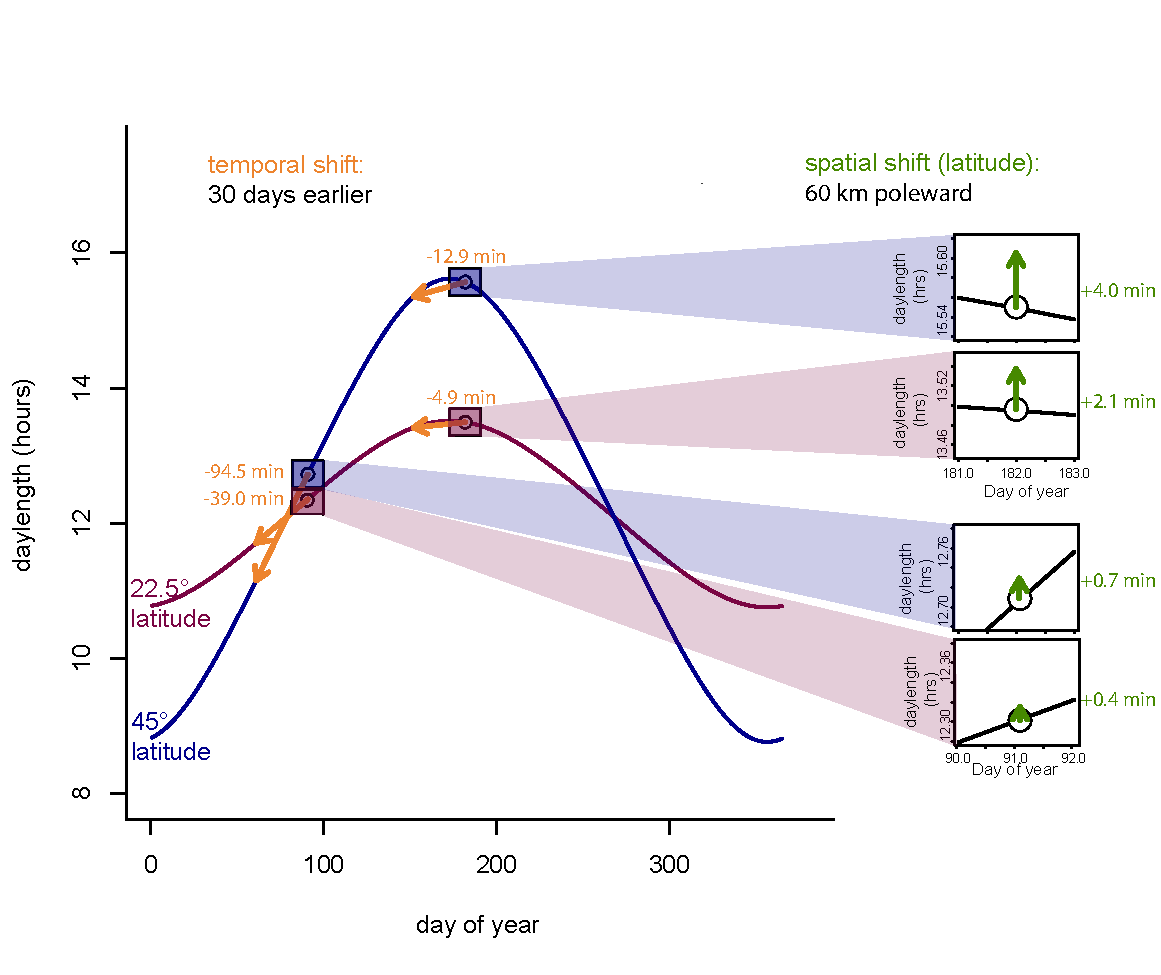
\includegraphics{photo_spacetime_v4b_newcolors.pdf} %
\caption{\textbf{Temporal (i.e., phenological) shifts in activity yield larger changes in experienced photoperiod compared to spatial (i.e., latitudinal) shifts} on the same day of year, due to patterns in photoperiod variation with latitude and by day of year. Here, we show this variation at two latitudes (22.5$^{\circ}$, 45$^{\circ}$), using hypothetical spatial and temporal shifts. These shifts are based on observed rates with recent global warming: for spatial shifts, 6-17 kilometers per decade, or approximately 0.5-1.5$^{\circ}$ in 100 years \citep{parmesan2003,parmesan2006}; for temporal shifts, 3 days per decade, or 30 days in 100 years \citep{parmesan2006,chen2011}. These potential, plausible shifts highlight the greater magnitude in daylength changes from temporal shifts in the early spring, close to the vernal equinox (e.g., day of year 91), versus close to the summer solstice (e.g., day of year 182) at temperate latitudes.  It is also apparent that early spring temporal shifts at high latitudes result in more extreme changes in daylength than shifts at lower latitudes (e.g., a temporal shift 30 days earlier results in a reduction in daylength of 94.5 minutes at 45$^{\circ}$ versus 39.5 minutes at 22.5$^{\circ}$).}
 \label{fig:spacetime}%
 \end{figure}
 
 \begin{figure}[h]
\centering
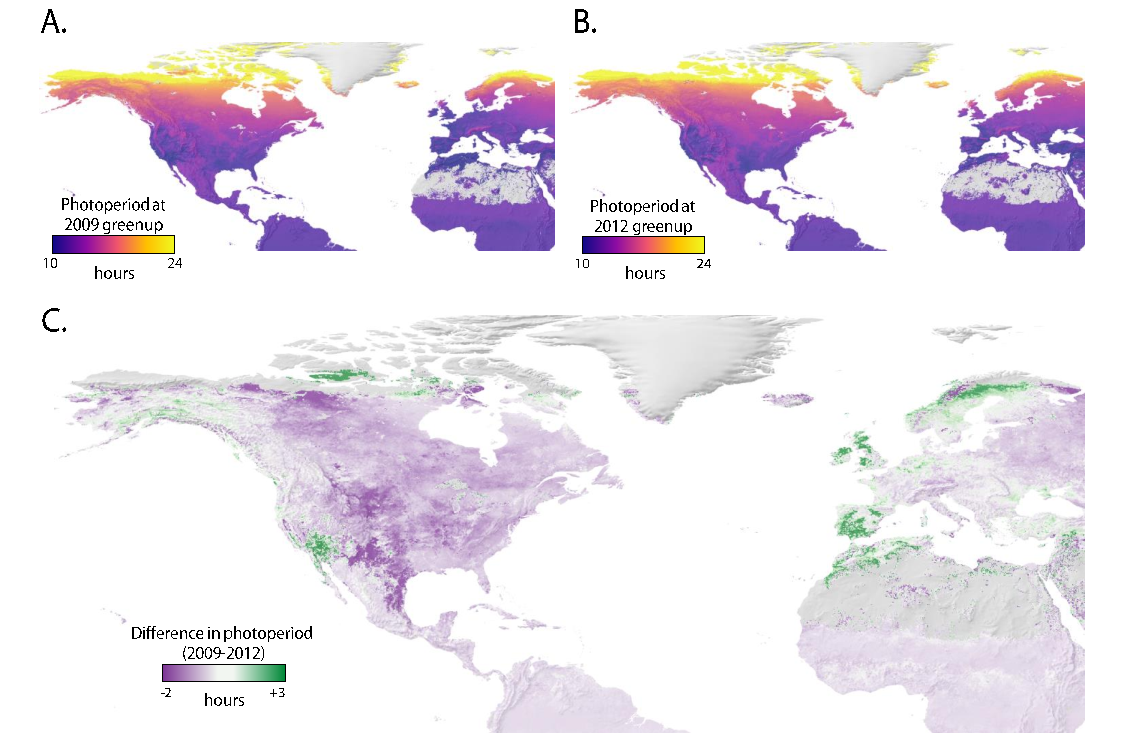
\includegraphics{Greenup_corr_sm_leg.pdf} %2009 greenup
\caption{\textbf{Photoperiod on `green-up' date varies over space and between years}. `Green-up' date is the beginning of seasonal greening, identified by satellite remote sensing measurements, taken regularly throughout the year, of concentrations of green leaf vegetation. Hours of daylight are shown on the date of spring green-up (here from MODIS satellite data) across North America and Europe for an average (2009, A) and early (2012, B) North American start of spring. The differences between the years (in hours of daylength) are shown in (C). A negative difference signifies earlier green-up in 2012 versus 2009; a positive difference is the result of later green-up in 2012 compared with 2009. See ``Quantifying and mapping differences in green-up across the United States and Europe'' in Methods S1 of the \emph{Supporting Information} for additional details. }%
 \label{fig:greenup}%
 \end{figure}

\begin{figure}[h]
\centering
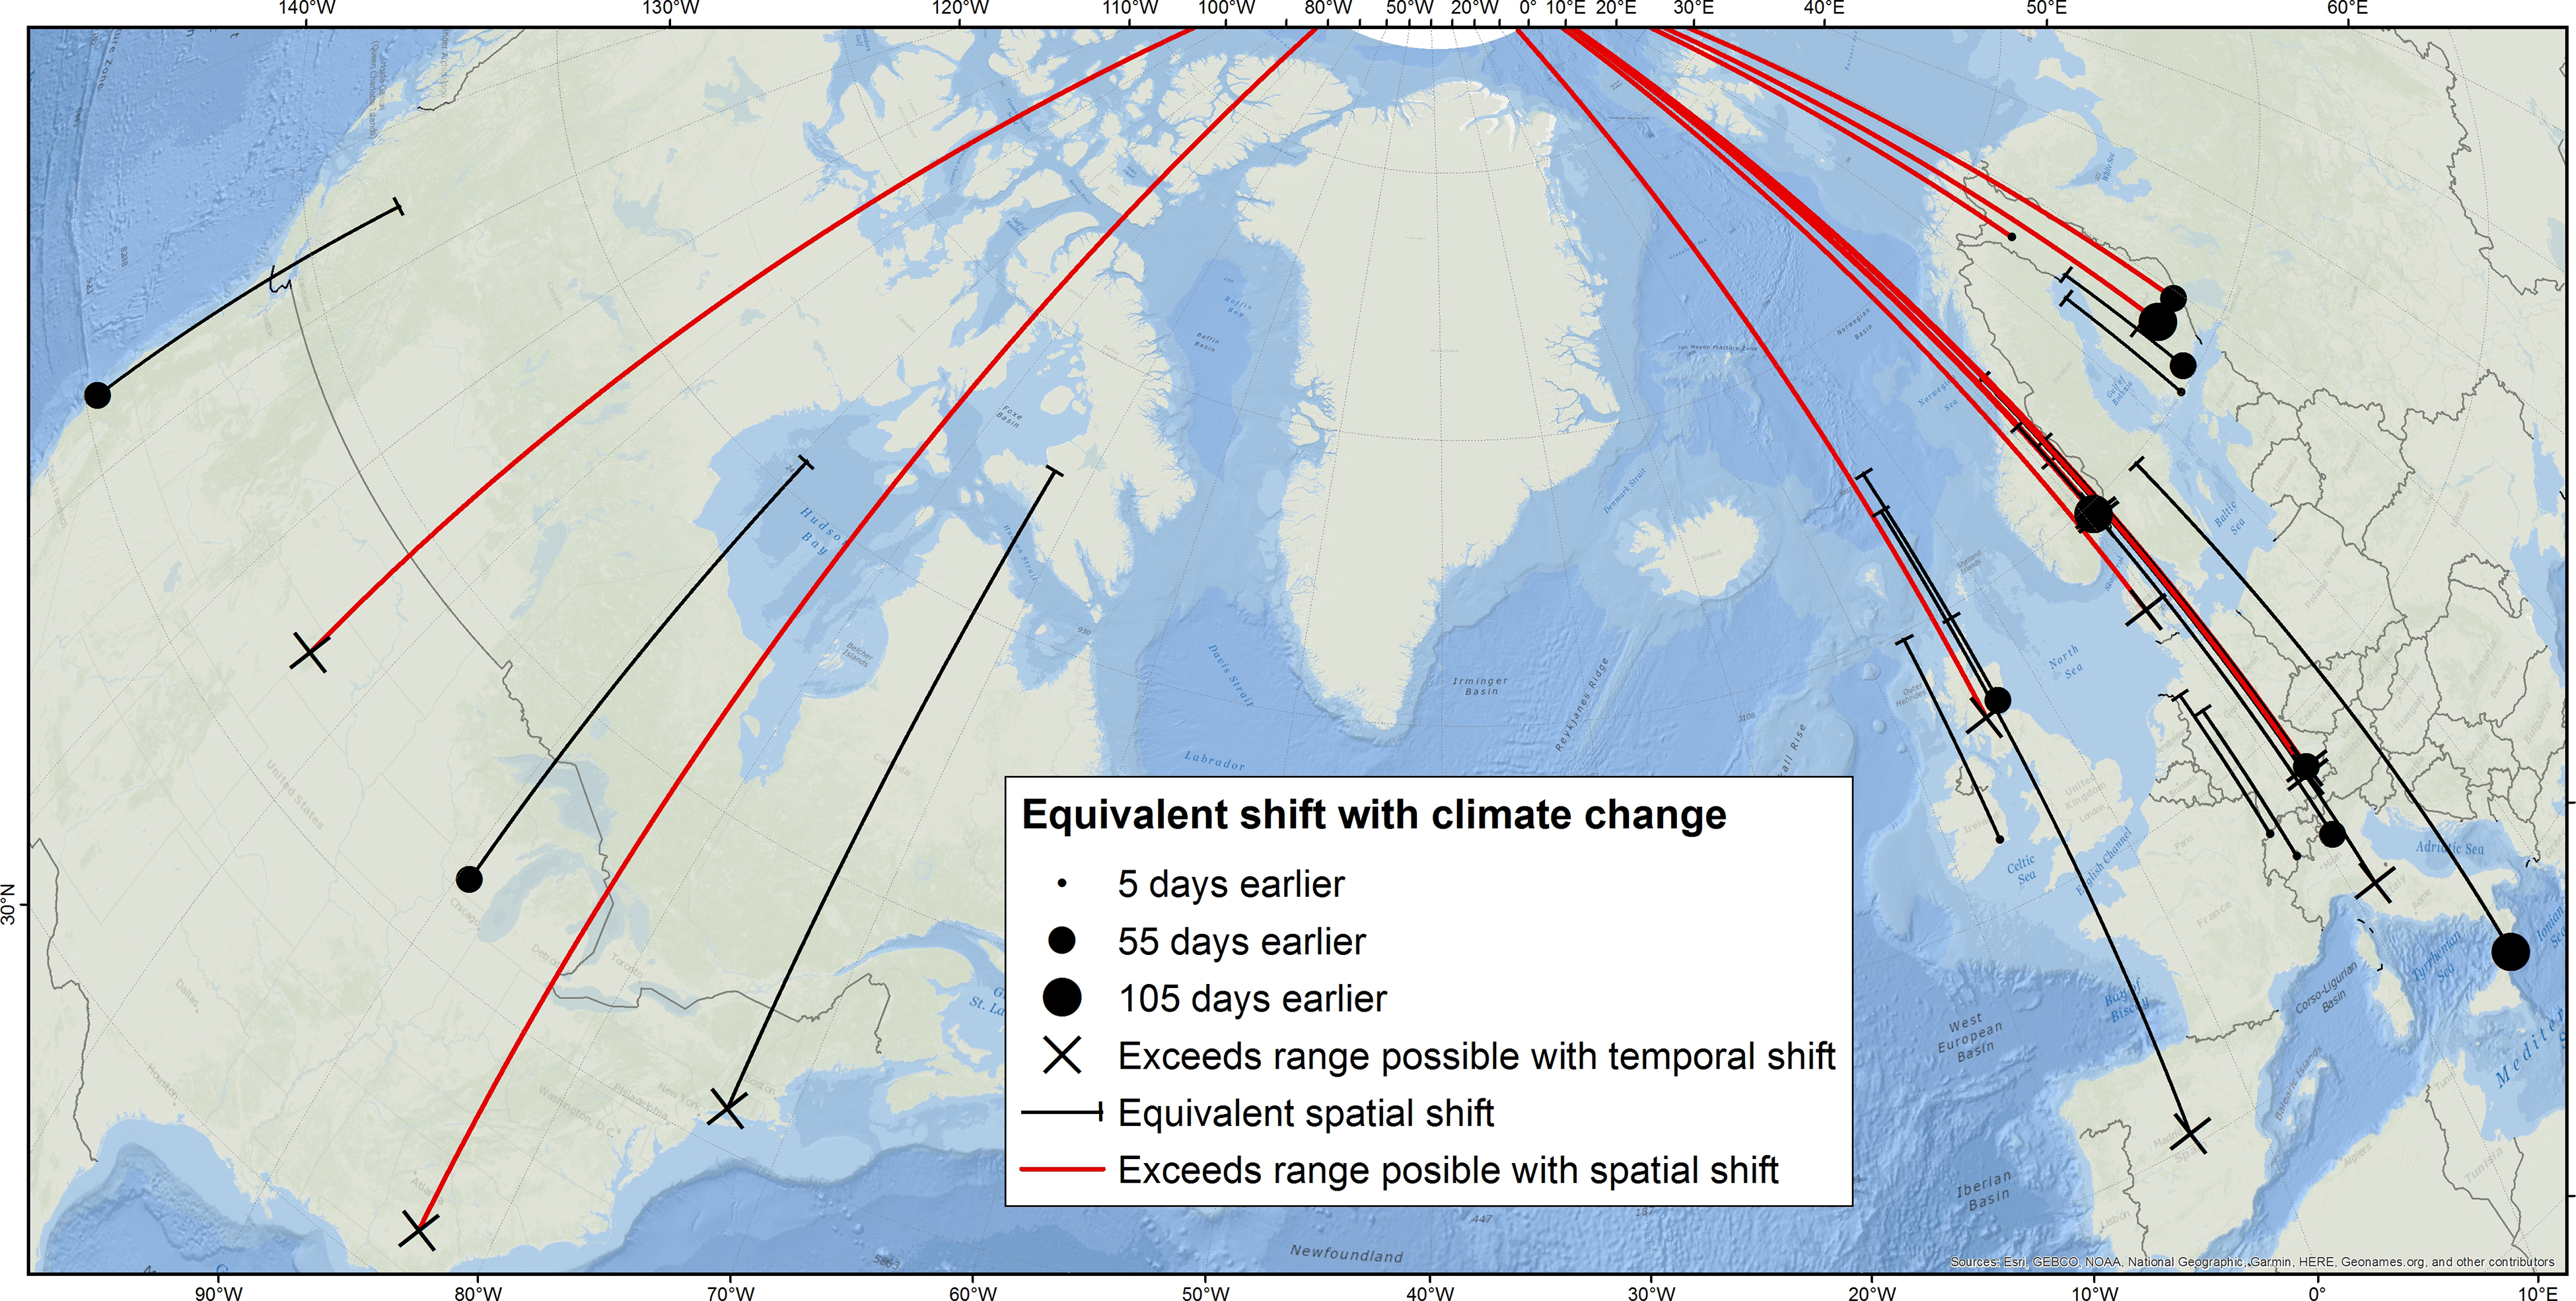
\includegraphics{ospree_photopmap_fromblake.jpg} 
\caption{\textbf{A map of experimental photoperiod treatments from a meta-analysis of woody plant spring phenology and their equivalent spatial and temporal shifts} demonstrates that many experiments manipulate photoperiod more dramatically than will occur with climate change. Mapped points (circles and Xes) are locations of experiments in \citet{wolkovich2019} that manipulated photoperiod (30 total experiments; see Box 1). In 11 out of 30 cases, the difference between experimental treatments exceeded the range in photoperiod experienced across the entire year at the study latitude (Xs; circles mark temporal shifts within a possible range). Note that many studies occur at high latitudes, which experience a wide range of photoperiod across the year. In 13 out of 30 cases, the experimental treatment differences exceeded the photoperiod change that would be experienced with a latitudinal shift of up to 40$^{\circ}$ (red lines; black lines represent spatial shifts within a possible range). See ``Mapping temporal and spatial shifts in space and time'' in Methods S1 of the \emph{Supporting Information} for additional details. }
 \label{fig:photomap}
 \end{figure}


\begin{figure}[h]
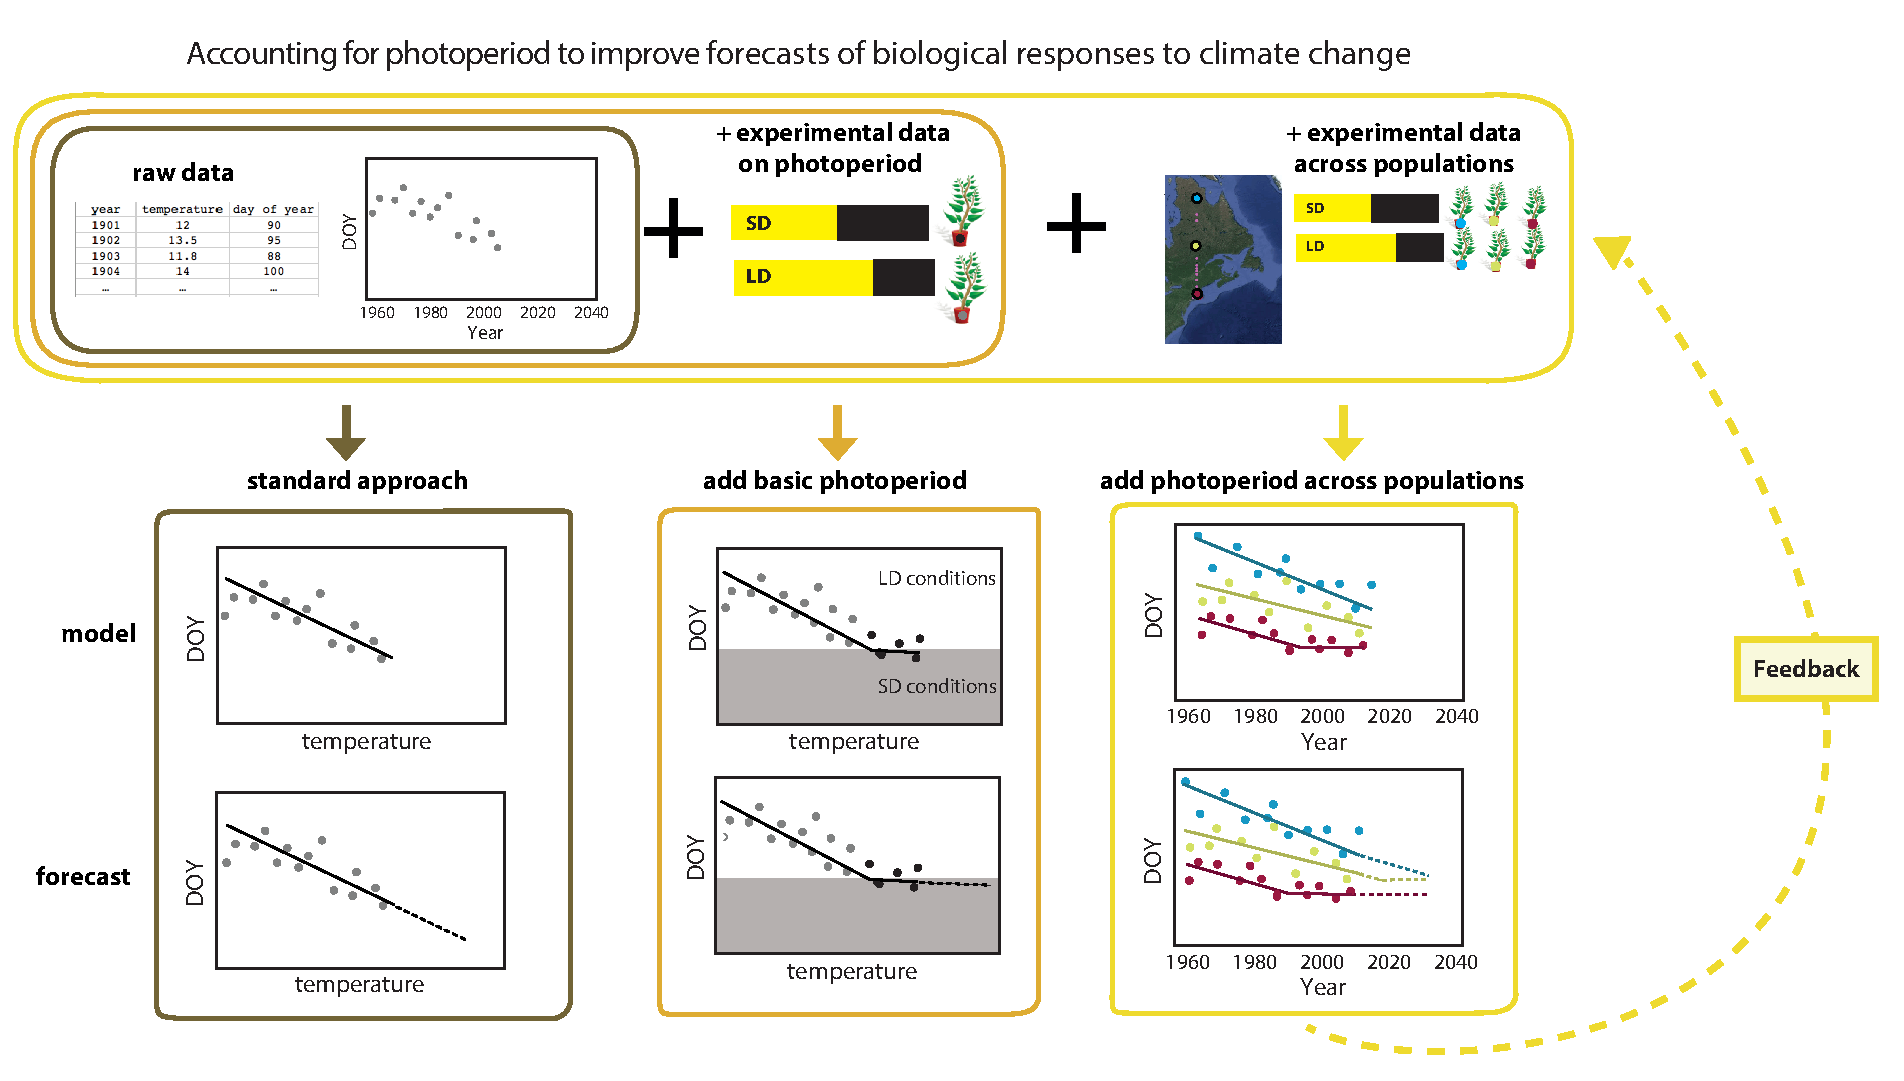
\includegraphics{photocondiag6.pdf} 
\caption{\textbf{Conceptual diagram of how to include photoperiod in forecasting biological responses to climate change}. Current approaches for forecasting spring phenology with climate change frequently rely on linear relationships between historical temperature data and observed dates of spring phenology (left panels). Adding responses to photoperiod, which may operate as threshold responses to short days (SD) versus long days (LD, see `photoperiod sensitivity' in Table 1 and Box 2 for details), will alter these forecasts (center panel) in ways that differ across species with divergent threshold photoperiods. Other factors that interact with photoperiod, such as population-level variation in photoperiod responses, can be incorporated into forecasts to further improve their accuracy (right panel).}
 \label{fig:condiag}
 \end{figure}
\clearpage

 
 \section*{Box 1. Are photoperiod effects widespread? A case study of woody plant spring phenology}
\par Photoperiod responses are well-studied in woody plant phenology, making this a useful case study to consider climate change-induced shifts in photoperiod. Spring woody plant phenology in particular has critical implications for global carbon cycling and feedbacks to the climate system \citep{richardson2013}, and has been at the center of an important and controversial debate on the relative effects of photoperiod versus temperature on phenology \citep[e.g.,][]{fu2019,chuine2010,koerner2010a,koerner2010b}. 

\par Experimental growth chamber studies have shown that photoperiod is an important cue for spring budburst phenology in woody plants \citep[e.g.,][]{flynn2018,Basler:2014aa,Heide:1993a}. These experiments often manipulate photoperiod in combination with temperature to address basic questions about how these two environmental conditions act as biological cues. Temperature has a dual role in regulating woody plant phenology: chilling---the prolonged exposure to cold temperatures after growth cessation in the fall---is required to initiate budburst, and forcing---prolonged exposure to warm temperatures---is required for budburst to occur. Different photoperiod treatments are typically applied during the forcing treatment phase in growth chamber experiments \citep[e.g.,][]{Laube:2014a,Spann:2004aa,Falusi:1990aa,HEIDE:1977aa,Campbell:1975aa}. 

\par Woody plant growth chamber studies have been conducted for decades, but have only recently been synthesized to show that photoperiod sensitivity is widespread, with large variation across studies and species. These studies were aggregated in Observed Spring Phenology Responses in Experimental Environments (OSPREE), a new database of plant growth chamber studies that manipulate photoperiod and temperature to measure plant phenological responses, such as budburst and flowering \citep{wolkovich2019}. The database includes studies that manipulate photoperiod (by applying treatments with different daylength durations, applying long-day versus short-day conditions for different lengths of time, and/or applying varying versus constant photoperiods) and temperature (by imposing different chilling and/or forcing treatments). The OSPREE database spans 201 woody plant species; all experiments in the database use dormant plant tissue (grown in greenhouses or taken directly from the field) exposed to experimental conditions for which we could identify forcing, photoperiod, and chilling treatments quantitatively. See Methods S1 of the \emph{Supporting Information}, \citet{ettinger2020}, and \citet{wolkovich2019} for details. 


\par Growth chamber experiments in OSPREE suggest that the dominant photoperiod response in woody plant species is earlier and more rapid budburst with longer days \citep [e.g., ][]{Caffarra:2011a}. Thirty of the 72 studies in the OSPREE database included two or more different photoperiod treatments. Of these, 26 (87\%) found significant photoperiod main effects or significant interactive effects with temperature (i.e., photoperiod x temperature effects), across 176 species (Table S1). Main effects included responses such as growth \citep[e.g., higher growth rates with longer days][]{Ashby:1962aa} and reproduction \citep[e.g., increased flowering with longer days][]{Heide:2012aa}. 


\par Growth chamber experiments highlight that responses to photoperiod vary depending on temperature conditions. For example, an accelerated advance of budburst was observed under long versus short days with low chilling, relative to bubdburst with high chilling in \emph{Betula payrifera} \citep[][see Fig. Box 1-1]{Hawkins:2012}. Similarly, across species, as chilling accumulates from winter to spring, sensitivity to both forcing and photoperiod sensitivity can decrease \citep{malyshev2018}. Frequently, long photoperiods can compensate for low amounts of chilling \citep{Caffarra:2011b,Myking:1995,Heide:1993}.%or low forcing?
\par Woody plant growth chamber experiments also demonstrate that, though photoperiod responses are common, they are variable, as shown in Fig. Box 1-1. Responses to photoperiod differ by species \citep[e.g.,][]{flynn2018,zohner2016,Basler:2014aa,Basler:2012,Howe:1996,Heide:1993a}.
For example, with longer chilling treatments some species seem insensitive to daylength \citep[e.g., \emph{Hammamelis} spp., \emph{Prunus} spp.,][]{zohner2016}, whereas others seem to be highly sensitive to daylength (e.g. \emph{Fagus} spp., Fig. \ref{fig:fagus}A), even with long chilling treatments \citep{zohner2016}. In addition, some species demonstrate a response to photoperiod opposite to that typically observed: \emph{Tilia}, for example, showed delayed budburst with longer daylengths \citep[see Fig. Box 1-1,][]{Ashby:1962aa}.
Photoperiod sensitivity also varies by population and ecotype (e.g., Fig. Box 1-1). For example, photoperiod effects on budburst were more significant for lower latitude populations of \emph{Betula pendula} and \emph{B. pubescens} \citep{Partanen:2005aa}. 

\makeatletter
\renewcommand{\thefigure}{Box 1-\@arabic\c@figure}
\makeatother
\setcounter{figure}{0}
\begin{figure}[h]
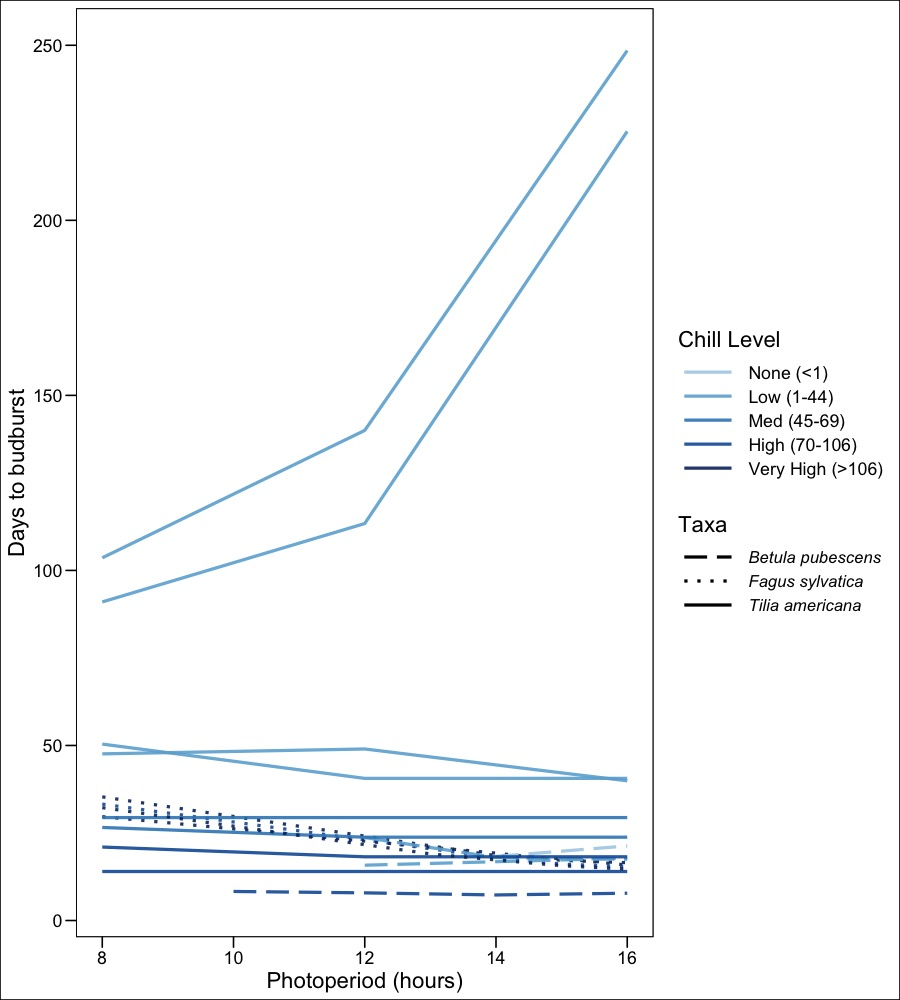
\includegraphics{Photo_curv_version2blue.jpeg} 
\caption{\textbf{ Nonlinearities in phenological responses to daylength} are apparent in spring woody plant phenology experiments. Shown are responses from all experiments  from \citet{wolkovich2019}in which three or more photoperiod treatment levels were applied. The shape of the response curves for \textit{Betula pubescens} \citep{Caffarra:2011b}, \textit{Fagus sylvatica} \citep{Heide:1993a} and \textit{Tilia americana} \citep{Ashby:1962aa} differ depending on the amount of winter chilling received \citep[measured in Chill portions,][with darker blue indicating more chilling]{fishman1987}. Species and chilling levels with multiple lines represent plant material from different populations. See ``Nonlinearities in phenological responses to daylength'' in Methods S1 of the \emph{Supporting Information} for additional details.}

\label{fig:photocurve}
\end{figure}

\begin{figure}[h]
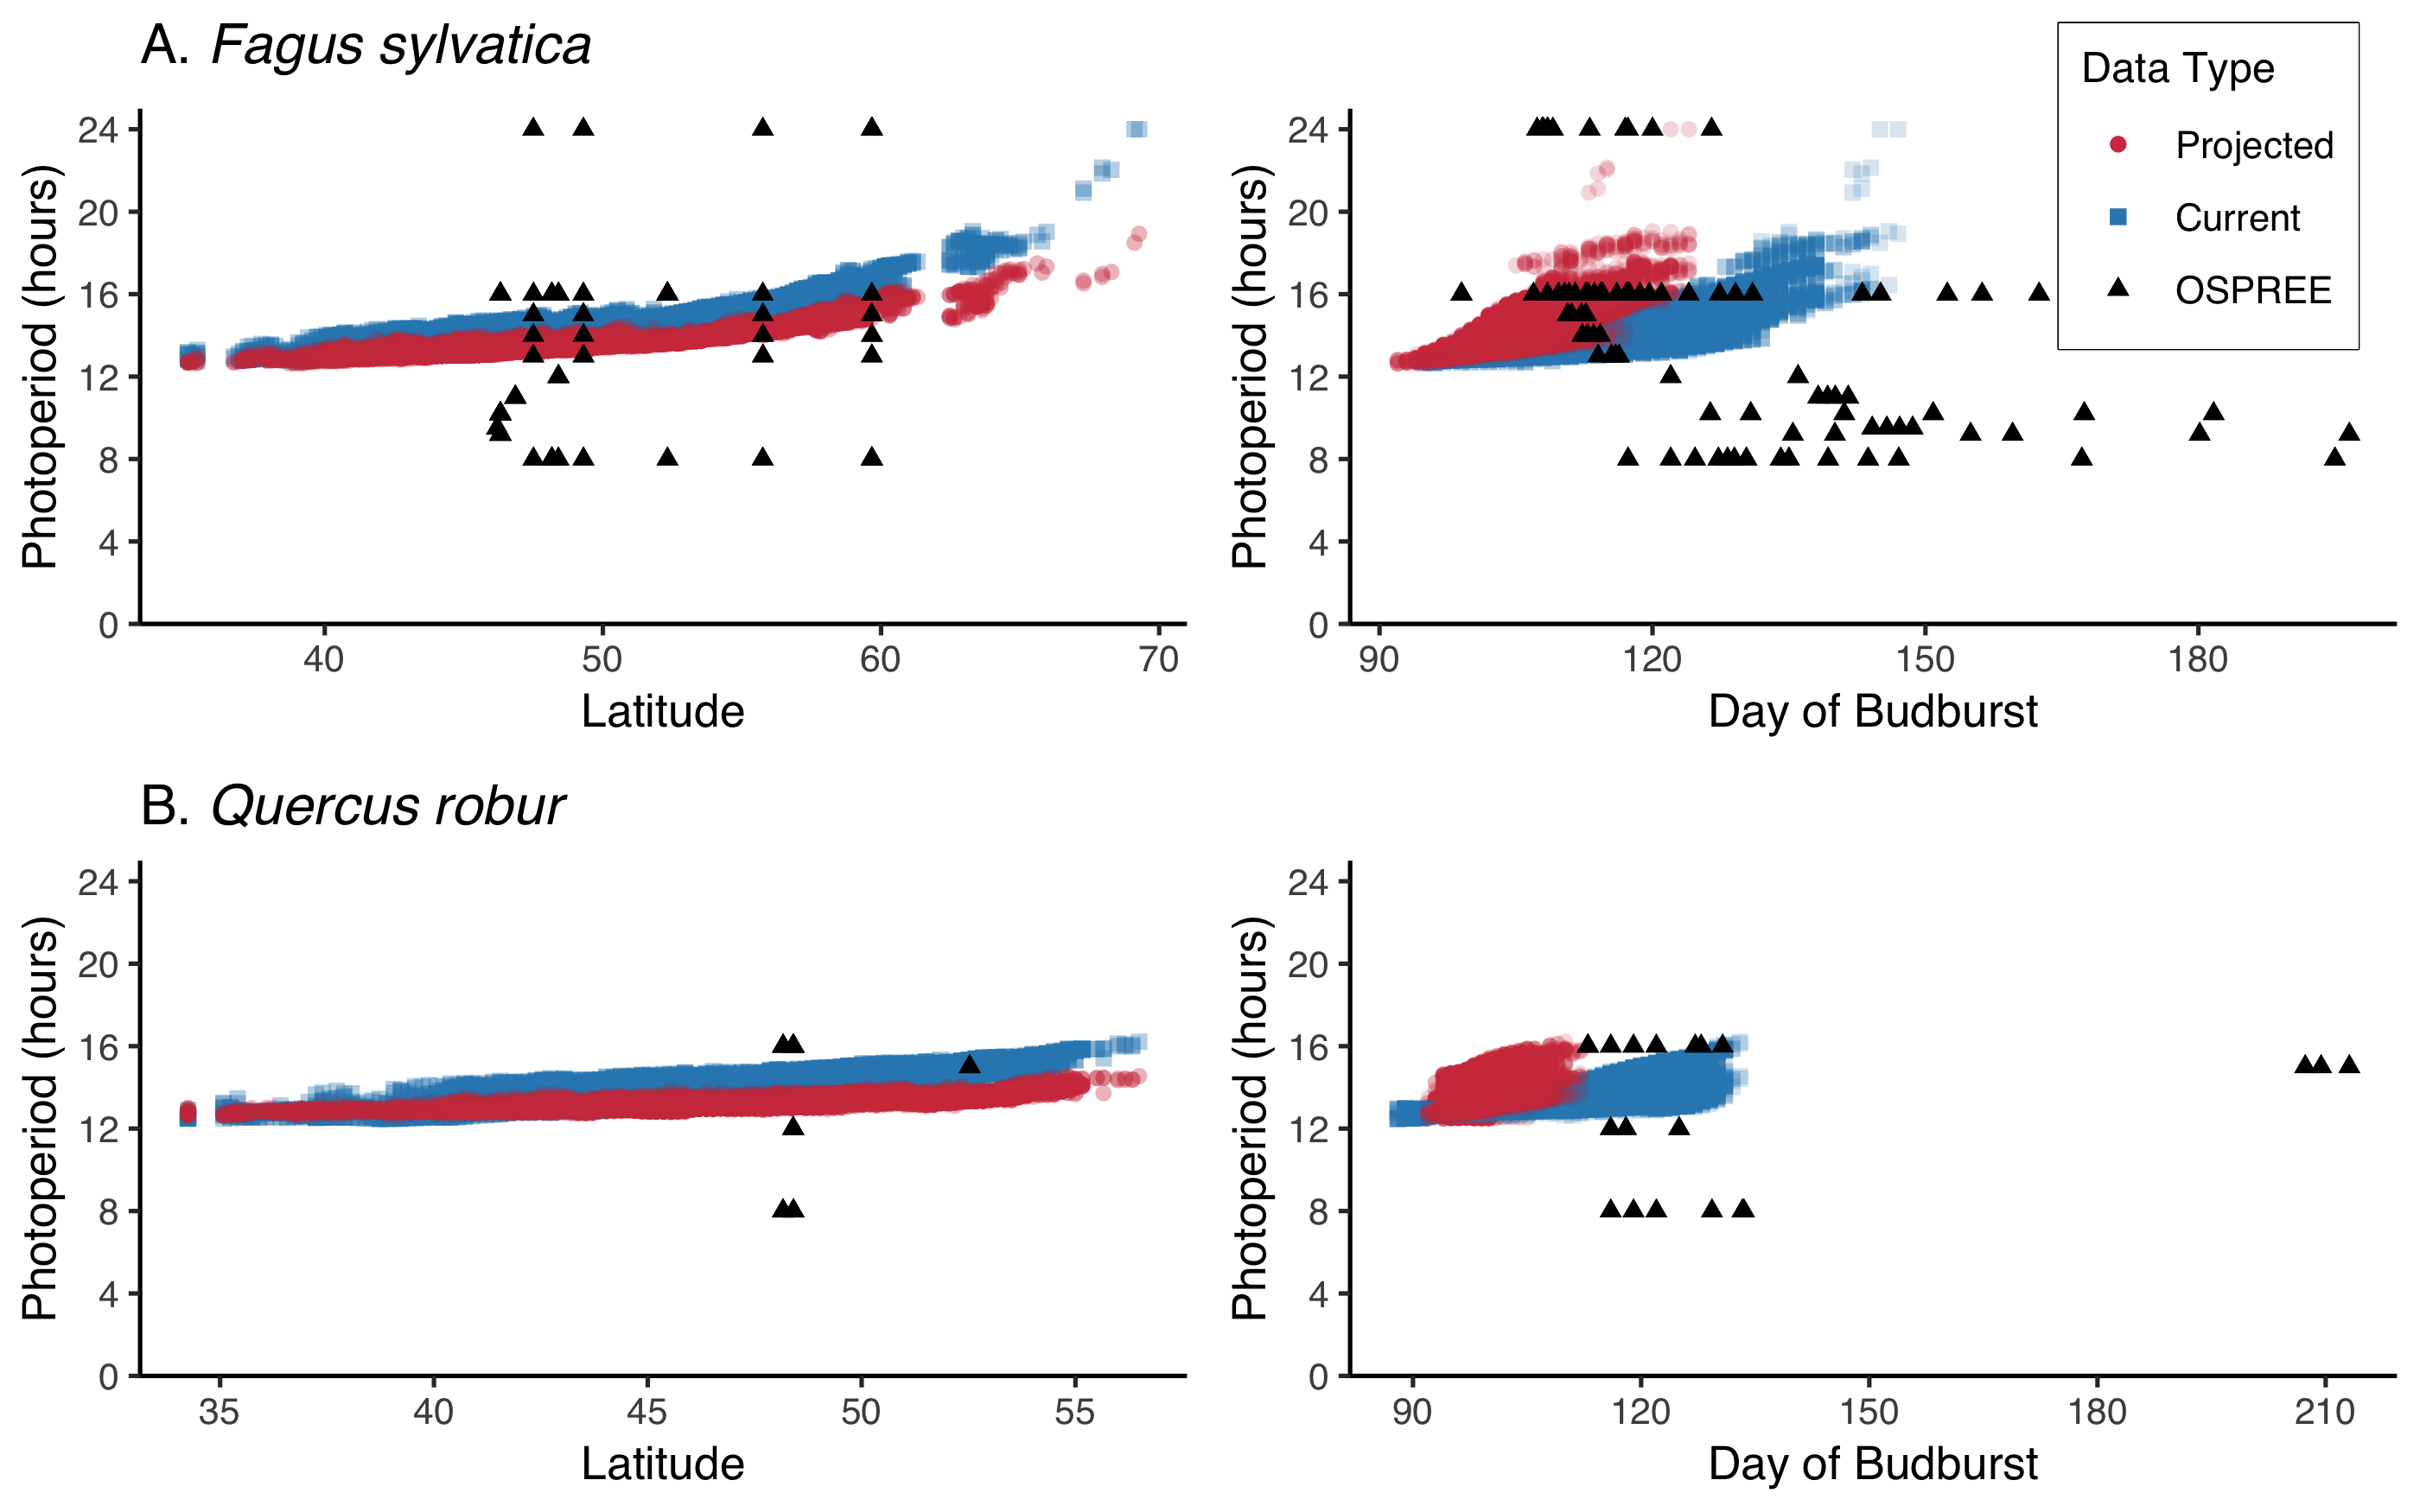
\includegraphics{2D_actual_combined.png} 
\caption{\textbf{Experienced photoperiods in growth chamber experiments differ from those in the natural world}, shown here by latitude (left panels) and by day of budburst (right panels) for \emph{Fagus sylvatica} (A, upper panels) and \emph{Quercus robur} (B, lower panels). Triangles show experimental treatments of photoperiod in \citet{wolkovich2019}. To illuminate potential gaps between experiments and the natural world, we show the photoperiod when budburst occurs in its current (1981-2000) and projected ranges \citep[2081-2100, using the A1Fi Phenofit scenario, see][]{duputie2015}. We scaled the days to budburst for all data points in \citet{wolkovich2019} by adding the day of budburst from the first Phenofit observation. See ``Comparing shifts in experienced photoperiod in experiments to those in the natural world with climate change'' in Methods S1 of the \emph{Supporting Information} and \citet{duputie2015} for additional details.} 
 \label{fig:fagus}
 \end{figure}
 
\clearpage 
\section*{Box 2. Dominant models of how photoperiod affects spring woody plant phenology}
\par The cues and molecular pathways underlying photoperiod sensitivity are poorly understood for most organisms, even in relatively well-studied phenophases and taxa, such as spring budburst in woody plants \citep{ding2016}. Decades of growth chamber experiments demonstrate that three main cues---chilling, forcing, and photoperiod---control spring budburst for woody species \citep{flynn2018, zohner2016,Heide:2008aa}, with many models suggesting a dominant role of forcing in most natural conditions. Forcing requirements, however, appear to increase given shorter photoperiods or lower chilling \citep{Caffarra:2011qf,chuine2010}. Research has yet to fully tease out effects of these three cues, their interactions, and their prevalence;  photoperiod responses appear variable across species and populations, as well as with different chilling treatments (see Box 1). Not surprisingly, there is currently little agreement on the underlying model for how photoperiod affects spring phenology for most species \citep{chuine2016,hanninen2019}. More physiological research will likely be necessary for major advances, as understanding the exact cellular pathways through which chilling, forcing, and photoperiod act appears increasingly critical to accurate modelling \citep{vanderschoot2014,hanninen2019}. 

\par Additional cellular and molecular studies may quickly advance understanding and scale up to improved photoperiod models. While our understanding of how plants interpret photoperiod at the molecular-level comes from few species, largely from studies of flowering in the model plant \emph{Arabidopsis thaliana} \citep[e.g.,][]{suarez2001} and fall budset in woody plant species \citep[e.g.,][]{Howe:1996}, these studies have proved useful across other species. For example, the `external coincidence model' \citep[where plants sense light via blue light receptors and phytochromes, then interpret photoperiod through a coordinated response to light in relation to the time of day, see][]{lagercrantz2009} has been most widely studied in \emph{Arabidopsis}, but appears to be a relevant mechanism for photoperiod responses in diverse perennial and woody plant species \citep{Singh:2017,petterle2013,andres2012,kobayashi2007,davis2002,bastow2002,bunning1936}. The model proposes the existence of a circadian rhythm of light sensitivity, in which the night-phase is sensitive to light and the day-phase is insensitive to light. As days get longer in the spring, daylight illuminates the light sensitive phase, triggering a response. This provides a clear mechanistic pathway to build into models \citep{Burghardt2015}. 

\par We expect progress on spring phenology will benefit from similar physiological research that spans the molecular to whole-plant levels. To date, little is known about the genetic pathways responsible for the light-sensing apparatuses involved in spring budburst, and how they may vary across species or populations. Some genes have been identified that play a role in coordinating budburst in poplar (\emph{Populus} spp.), and may occur in other woody species as well. Many similarities exist between the proposed regulatory networks of vegetative growth in \emph{Populus} and those controlling floral initiation in \emph{Arabidopsis}, \citep{ding2016}. For example, vegetative growth and inhibition of budset are promoted by the FLOWERING LOCUS T2 (FT2) gene, a homolog of \emph{Arabidopsis thaliana} gene FLOWERING LOCUS (FT). FT2 expression appears to be controlled by a pathway that is effective in long days and warm temperatures, marking the onset of the growing season \citep{Hsu:2011}. Its loss of expression in autumn, when the days are getting shorter, is associated with the onset of dormancy \citep{glover2014}.

\par Efforts to better map the genetic and cellular pathways of spring phenology combined with common garden studies can provide a powerful method to test mechanistic understanding and improve models \citep[e.g.,][]{Burghardt2015,fournier2016}. Here we have mainly outlined how to combine growth chamber studies with long-term data to improve models and forecasting; a greater physiological understanding of at least a few species will likely also be necessary for generating robust predictions with climate change.

%%%%%%%%%%%%%%%%%%%%%%%%%%%%%%%%%%%%%%%%
\end{document}
%%%%%%%%%%%%%%%%%%%%%%%%%%%%%%%%%%%%%%%%
